\newcommand*{\BeamerSuffix}{-pres}
\newcommand*{\TransSuffix}{-slides}
\documentclass{beamer}
\setbeamertemplate{navigation symbols}{}

\usepackage{movie15}
\usepackage{amssymb,amsmath}
\usepackage{hyperref}
\usepackage{natbib} 
\usepackage{pgf} 
\usepackage{mathtools}
\usepackage{tikz}
\usepackage{bbm}

\usetheme{Madrid}	% clean, nice.  7/12 page numbers




%\newtheorem{example}{Example}

\newcommand{\expect}{\mathbb{E}}
\newcommand{\variance}{\mathrm{Var}}
\DeclareMathOperator*{\Var}{Var}
\newcommand{\covariance}{\mathrm{Cov}}
\DeclareMathOperator*{\Cov}{Cov}
\newcommand{\prob}{\mathrm{Pr}}
\newcommand{\zeroVec}{\mathbf{0}}
\newcommand{\zeroMat}{\mathbf{0}}
\newcommand{\onesVec}{\mathbf{1}}
\newcommand{\ident}{\mathbf{I}}
\newcommand{\deriv}{\mathrm{d}}
\newcommand{\transpose}{\top}
\newcommand{\costDeriv}[1]{\overline{#1}}
\newcommand{\lossDeriv}{\costDeriv}
\newcommand{\normal}{\mathcal{N}}
\newcommand{\data}{\mathcal{D}}

\newcommand{\dataIdx}{i}
\newcommand{\featIdx}{j}
\newcommand{\dimIdx}{\featIdx}
\newcommand{\paramIdx}{\dimIdx}
\newcommand{\hidIdx}{i}
\newcommand{\classIdx}{k}
\newcommand{\outputIdx}{k}
\newcommand{\classIdxTwo}{\ell}
\newcommand{\featIdxTwo}{j^\prime}
\newcommand{\nfeat}{D}
\newcommand{\ndim}{\nfeat}
\newcommand{\ndata}{N}
\newcommand{\numClasses}{K}
\newcommand{\nout}{\numClasses}
\newcommand{\layerIdx}{\ell}
\newcommand{\numLayers}{L}
\newcommand{\nhid}{M}
\newcommand{\timeIdx}{t}
\newcommand{\ntime}{T}
\newcommand{\contextLen}{K}


\newcommand{\inputIJ}[2]{x^{(#1)}_{#2}}
\newcommand{\inputI}[1]{{\bf x}^{(#1)}}
\newcommand{\inputJ}[1]{x_{#1}}
\newcommand{\inputVec}{{\bf x}}
\newcommand{\inputVecT}[1]{\inputVec^{(#1)}}
\newcommand{\inputVecI}[1]{\inputVec^{(#1)}}
\newcommand{\inputUni}{x}
\newcommand{\inputUniI}[1]{x^{(#1)}}
\newcommand{\inputUniT}[1]{x^{(#1)}}
\newcommand{\inputMatrix}{\mathbf{X}}
\newcommand{\inputMatrixT}[1]{\inputMatrix^{(#1)}}
\newcommand{\targetI}[1]{t^{(#1)}}
\newcommand{\target}{t}
\newcommand{\targetK}[1]{\target_{#1}}
\newcommand{\targets}{\mathbf{t}}
\newcommand{\prediction}{y}
\newcommand{\predictionI}[1]{y^{(#1)}}
\newcommand{\predictionK}[1]{y_{#1}}
\newcommand{\predictionT}[1]{y^{(#1)}}
\newcommand{\predictions}{\mathbf{y}}
\newcommand{\predictionMatrix}{\mathbf{Y}}
\newcommand{\predictionMatrixT}[1]{\predictionMatrix^{(#1)}}
\newcommand{\intermediate}{z}
\newcommand{\intermediateI}[1]{\intermediate^{(#1)}}
\newcommand{\intermediateT}[1]{\intermediate^{(#1)}}
\newcommand{\intermediateK}[1]{\intermediate_{#1}}
\newcommand{\intermediates}{\mathbf{z}}
\newcommand{\intermediateMatrix}{\mathbf{Z}}
\newcommand{\intermediateMatrixT}[1]{\intermediateMatrix^{(#1)}}
\newcommand{\outIntermediate}{r}
\newcommand{\outIntermediateT}[1]{r^{(#1)}}
\newcommand{\outIntermediateK}[1]{\outIntermediate_{#1}}
\newcommand{\outIntermediates}{\mathbf{r}}
\newcommand{\outIntermediateMat}{\mathbf{R}}
\newcommand{\outIntermediateMatrix}{\mathbf{R}}
\newcommand{\outIntermediateMatrixT}[1]{\outIntermediateMatrix^{(#1)}}
\newcommand{\hiddenI}[1]{h_{#1}}
\newcommand{\hiddenT}[1]{h^{(#1)}}
\newcommand{\hiddenIT}[2]{h_{#1}^{(#2)}}
\newcommand{\hiddenLI}[2]{h_{#2}^{(#1)}}
\newcommand{\hiddens}{\mathbf{h}}
\newcommand{\hiddensL}[1]{\hiddens^{(#1)}}
\newcommand{\hiddensT}[1]{\hiddens^{(#1)}}
\newcommand{\hiddenMatrix}{\mathbf{H}}
\newcommand{\hiddenMat}{\hiddenMatrix}
\newcommand{\hiddenMatrixT}[1]{\hiddenMatrix^{(#1)}}
\newcommand{\hiddenMatL}[1]{\hiddenMat^{(#1)}}
\newcommand{\weights}{{\bf w}}
\newcommand{\weightsL}[1]{\weights^{(#1)}}
\newcommand{\weightJ}[1]{w_{#1}}
\newcommand{\weightLIJ}[3]{w^{(#1)}_{#2 #3}}
\newcommand{\weightLKI}[3]{w^{(#1)}_{#2 #3}}
\newcommand{\weightLJ}[2]{w^{(#1)}_{#2}}
\newcommand{\weightKJ}[2]{w_{#1 #2}}
\newcommand{\weightIJ}{\weightKJ}
\newcommand{\weightUni}{w}
\newcommand{\weightMat}{\mathbf{W}}
\newcommand{\weightMatL}[1]{\weightMat^{(#1)}}
\newcommand{\bias}{b}
\newcommand{\biasLI}[2]{\bias^{(#1)}_{#2}}
\newcommand{\biasLK}{\biasLI}
\newcommand{\biasL}[1]{\bias^{(#1)}}
\newcommand{\biasK}[1]{\bias_{#1}}
\newcommand{\biasJ}[1]{\bias_{#1}}
\newcommand{\biases}{\mathbf{b}}
\newcommand{\biasesL}[1]{\biases^{(#1)}}
\newcommand{\threshold}{r}
\newcommand{\featureJ}[1]{\psi_{#1}}
\newcommand{\featureVec}{{\boldsymbol \psi}}
\newcommand{\loss}{\mathcal{L}}
\newcommand{\lossI}[1]{\loss^{(#1)}}
\newcommand{\zeroOneLoss}{\loss_{\rm 0-1}}
\newcommand{\squaredErrorLoss}{\loss_{\rm SE}}
\newcommand{\crossEntropyLoss}{\loss_{\rm CE}}
\newcommand{\logisticCrossEntropyLoss}{\loss_{\rm LCE}}
\newcommand{\softmaxCrossEntropyLoss}{\loss_{\rm SCE}}
\newcommand{\hingeLoss}{\loss_{\rm H}}
\newcommand{\cost}{\mathcal{J}}
\newcommand{\regularizer}{\mathcal{R}}
\newcommand{\lrate}{\alpha}
\newcommand{\learningRate}{\lrate}
\newcommand{\featureMap}{{\boldsymbol \psi}}
\newcommand{\featureMapJ}[1]{\psi_{#1}}
\newcommand{\sigmoid}{\sigma}
\newcommand{\logistic}{\sigmoid}
\newcommand{\activationFunction}{\phi}
\newcommand{\activationFunctionL}[1]{\activationFunction^{(#1)}}
\newcommand{\activationFunctionTwo}{\psi}
\newcommand{\parityFunction}{f_{\rm par}}
\newcommand{\function}{f}
\newcommand{\functionL}[1]{\function^{(#1)}}
\newcommand{\indicatorOf}[1]{\mathbbm{1}_{#1}}
\newcommand{\softmax}{\mathrm{softmax}}
\newcommand{\weightCost}{\lambda}
\newcommand{\genCost}{\mathcal{C}}
\newcommand{\momentumVec}{\mathbf{p}}
\newcommand{\momentumJ}[1]{p_{#1}}
\newcommand{\momentumParam}{\mu}
\newcommand{\genParams}{{\boldsymbol \theta}}
\newcommand{\genParamJ}[1]{\theta_{#1}}
\newcommand{\pData}{p_{\mathcal{D}}}
\newcommand{\bestPrediction}{\prediction_\star}

\newcommand{\obs}{\mathbf{x}}
\newcommand{\obsJ}[1]{x_{#1}}
\newcommand{\obsI}[1]{\obs^{(#1)}}
\newcommand{\pfn}{\mathcal{Z}}
\newcommand{\happiness}{H}
\newcommand{\latents}{\mathbf{z}}

\newcommand{\state}{\mathbf{s}}
\newcommand{\stateT}[1]{\state_{#1}}
\newcommand{\act}{\mathbf{a}}
\newcommand{\actT}[1]{\act_{#1}}
\newcommand{\reward}{r}
\newcommand{\policy}{\pi}
\newcommand{\policyParams}{\boldsymbol{\theta}}
\newcommand{\policyTh}{{\policy_{\policyParams}}}
\newcommand{\MDP}{\mathcal{M}}
\newcommand{\rollout}{\tau}
\newcommand{\expectedReturn}{R}

\newcommand{\discReturn}{G}
\newcommand{\discFactor}{\gamma}
\newcommand{\valueFunc}{V}
\newcommand{\valueFuncPi}{\valueFunc^{\policy}}
\newcommand{\valueFuncPiTh}{\valueFunc^{\policyTh}}
\newcommand{\qFunc}{Q}
\newcommand{\qFuncPi}{\qFunc^{\policy}}
\newcommand{\optPolicy}{\policy^*}
\newcommand{\optQ}{\qFunc^*}

\newcommand{\subspace}{\mathcal{S}}
\newcommand{\projectedInput}{\tilde{\inputVec}}
\newcommand{\projectedInputI}[1]{\projectedInput^{(#1)}}
\newcommand{\codeVec}{\mathbf{z}}
\newcommand{\codeVecI}[1]{\codeVec^{(#1)}}
\newcommand{\dataMean}{\boldsymbol{\mu}}
\newcommand{\dataCov}{\boldsymbol{\Sigma}}
\newcommand{\pcaVec}{\mathbf{u}}

\newcommand{\featureMatrix}{{\boldsymbol \Psi}}
\newcommand{\smootherMatrix}{{\boldsymbol \Omega}}
\newcommand{\smootherMatrixEntry}{\Omega}
\newcommand{\hypothesis}{\mathcal{H}}
\newcommand{\priorMean}{\mathbf{m}}
\newcommand{\priorCov}{\mathbf{S}}
\newcommand{\priorVar}{\eta}
\newcommand{\postMean}{\boldsymbol{\mu}}
\newcommand{\postCov}{\boldsymbol{\Sigma}}
\newcommand{\predMean}{\mu_{\rm pred}}
\newcommand{\predVar}{\sigma^2_{\rm pred}}
\newcommand{\predStd}{\sigma_{\rm pred}}


\newcommand{\given}{\,|\,}
\newcommand{\TODO}[1]{{\color{red} {\bf [[#1]]}}}
\newcommand{\high}[1]{{\color{blue}{#1}}}



\newcommand{\naive}{na{\"\i}ve }





























%\newcommand{\Perp}{\perp\!\!\! \perp}


\newcommand{\Ep}[2]{\ensuremath{E_{#1}\left[{#2}\right]}}
\def\hpY{\mathbf{\bar{\beta}}}

\newcommand{\gaus}[2]{\mathcal{N}\left({#1};\,{#2}\right)}

\newcommand{\comment}[1]{}

\newcommand{\trace}{\text{trace}}
%\newcommand{\det}{\text{det}}

%\newcommand{\bm}{{\mathbf{m}}}
\newcommand{\loss}{{\cal L}}
\newcommand{\cG}{{\cal G}}
\newcommand{\cV}{{\cal V}}
\newcommand{\cE}{{\cal E}}
\newcommand{\cP}{{\cal P}}
\newcommand{\X}{{\cal X}}
\newcommand{\Y}{{\cal Y}}
\newcommand{\bK}{\mathbf{K}}
\newcommand{\bX}{\mathbf{X}}
\newcommand{\bY}{\mathbf{Y}}
\newcommand{\bk}{\mathbf{k}}
\newcommand{\bx}{\mathbf{x}}
\newcommand{\by}{\mathbf{y}}
\newcommand{\bhy}{\hat{\mathbf{y}}}
\newcommand{\bty}{\tilde{\mathbf{y}}}
\newcommand{\bG}{\mathbf{G}}
\newcommand{\bI}{\mathbf{I}}
\newcommand{\bg}{\mathbf{g}}
\newcommand{\bS}{\mathbf{S}}
\newcommand{\bs}{\mathbf{s}}
\newcommand{\bM}{\mathbf{M}}
\newcommand{\bw}{\mathbf{w}}
\newcommand{\eye}{\mathbf{I}}
\newcommand{\bU}{\mathbf{U}}
\newcommand{\bV}{\mathbf{V}}
\newcommand{\bW}{\mathbf{W}}
\newcommand{\bn}{\mathbf{n}}
\newcommand{\bv}{\mathbf{v}}
\newcommand{\bq}{\mathbf{q}}
\newcommand{\bR}{\mathbf{R}}
\newcommand{\bi}{\mathbf{i}}
\newcommand{\bj}{\mathbf{j}}
\newcommand{\bp}{\mathbf{p}}
\newcommand{\bt}{\mathbf{t}}
\newcommand{\bJ}{\mathbf{J}}
\newcommand{\bu}{\mathbf{u}}
\newcommand{\bB}{\mathbf{B}}
\newcommand{\bD}{\mathbf{D}}
\newcommand{\bz}{\mathbf{z}}
\newcommand{\bP}{\mathbf{P}}
\newcommand{\bC}{\mathbf{C}}
\newcommand{\bA}{\mathbf{A}}
\newcommand{\bZ}{\mathbf{Z}}
\newcommand{\bff}{\mathbf{f}}
\newcommand{\bF}{\mathbf{F}}
\newcommand{\bo}{\mathbf{o}}
\newcommand{\bc}{\mathbf{c}}
\newcommand{\bm}{\mathbf{m}}
\newcommand{\bT}{\mathbf{T}}
\newcommand{\bQ}{\mathbf{Q}}
\newcommand{\bL}{\mathbf{L}}
\newcommand{\bl}{\mathbf{l}}
\newcommand{\ba}{\mathbf{a}}
\newcommand{\bE}{\mathbf{E}}
\newcommand{\bH}{\mathbf{H}}
\newcommand{\bN}{\mathbf{N}}
\newcommand{\bd}{\mathbf{d}}
\newcommand{\br}{\mathbf{r}}
\newcommand{\be}{\mathbf{e}}
\newcommand{\bb}{\mathbf{b}}
\newcommand{\bh}{\mathbf{h}}
\newcommand{\bhh}{\hat{\mathbf{h}}}

\newcommand{\graph}{{\cal H}}
\newcommand{\bayes}{{\cal B}}
\newcommand{\cx}{{\cal X}}
\newcommand{\cg}{{\cal G}}
\newcommand{\cm}{{\cal M}}
\newcommand{\ci}{{\cal I}}
\newcommand{\ct}{{\cal T}}
\newcommand{\co}{{\cal O}}
\newcommand{\ck}{{\cal K}}
\newcommand{\cu}{{\cal U}}
\newcommand{\cv}{{\cal V}}
\newcommand{\ce}{{\cal E}}
\newcommand{\cf}{{\cal F}}
\newcommand{\cb}{{\cal B}}
\newcommand{\cq}{{\cal Q}}
\newcommand{\cd}{{\cal D}}

\newcommand{\btheta}{\boldsymbol{\theta}}
\newcommand{\bpi}{\boldsymbol{\pi}}
\newcommand{\bphi}{\boldsymbol{\phi}}
\newcommand{\bPhi}{\boldsymbol{\Phi}}
\newcommand{\bmu}{\boldsymbol{\mu}}
\newcommand{\bSigma}{\boldsymbol{\Sigma}}
\newcommand{\bGamma}{\boldsymbol{\Gamma}}
\newcommand{\bbeta}{\boldsymbol{\beta}}
\newcommand{\bomega}{\boldsymbol{\omega}}
\newcommand{\blambda}{\boldsymbol{\lambda}}
\newcommand{\bkappa}{\boldsymbol{\kappa}}
\newcommand{\btau}{\boldsymbol{\tau}}
\newcommand{\balpha}{\boldsymbol{\alpha}}
\def\bgamma{\boldsymbol\gamma}

\newcommand{\argmin}{\operatornamewithlimits{argmin}}

%\newcommand{\animal}[2]{\item[\bf #1] {\em #2}}
 \newcommand{\ikron}[1] {\bI\otimes #1}
  \newcommand{\val}{\bar{\bx}}
    \newcommand{\train}[1]{{\phi(\bx_{#1})}}
    \newcommand{\ikronval}[1]{(\ikron{\phi(\val_{#1}))}}
\newcommand{\ikronvalT}[1]{(\ikron{\phi(\val_{#1})^T)}}
\newcommand{\ikrontrainT}{(\ikron{\train{i}^T)}}
\newcommand{\ikrontrain}[1]{(\ikron{\train{#1})}}
\newcommand{\ikrontrainAT}{(\ikron{\phi(\bx)^T)}}
\newcommand{\ikrontrainA}{(\ikron{\phi(\bx))}}
  \newcommand{\half}{\frac{1}{2}}
  \newcommand{\con}{C^{(c)}}
    \newcommand{\ig}{\frac{1}{\gamma}}
      \newcommand{\Bi}{\bB^{-1}}
 \newcommand{\kernel}{\hat{\bK}}    
 \newcommand{\ikrontestT}{(\ikron{\test^T)}}
   \newcommand{\test}{\phi(\bx_*)}

% partial derivatives
 \newcommand{\pardev}[2]{\frac{\partial #1}{\partial #2}}
  \newcommand{\dev}[2]{\frac{d #1}{d #2}}
  \newcommand{\dw}{\delta\bw}
  
    \newcommand{\lab}{\mathcal{L}}
      \newcommand{\unlab}{\mathcal{U}}
      
      
  \newcommand{\ind}{1{\hskip -2.5 pt}\hbox{I}}
  
 \newcommand{\ff}[2]{   \cf_{\prec (#1 \rightarrow #2)}}
 \newcommand{\vv}[2]{   \cv_{\prec (#1 \rightarrow #2)}}
  \newcommand{\dd}[2]{   \delta_{#1 \rightarrow #2}}
    \newcommand{\ld}[2]{   \lambda_{#1 \rightarrow #2}}
    \newcommand{\en}[2]{  \bD(#1|| #2)}
       \newcommand{\ex}[3]{  \bE_{#1 \sim #2}\left[ #3\right]} 
       \newcommand{\exd}[2]{  \bE_{#1 }\left[ #2\right]} 
  
%  \newtheorem{theorem}{Theorem}
%\newtheorem{proposition}{Prop}
%\newtheorem{lemma}{Lemma}
%\newtheorem{lemma-ap}{Lemma}
%\newtheorem{definition}{Definition}
%\newtheorem{corollary}{Corollary}
%\newtheorem{claim}{Claim}
%\newtheorem{claim-ap}{Claim}
%\newcommand{\argmin}[1]{\underset{#1}{\mathrm{argmin}} \:}
\newcommand{\argmax}[1]{\underset{#1}{\mathrm{argmax}} \:}
\DeclareMathOperator*{\Max}{max}
\def\eop {{\noindent\framebox[0.5em]{\rule[0.25ex]{0em}{0.75ex}}}}

\newcommand{\tr}[1]{\ensuremath{\mathrm{tr}\left(#1\right)}}
\def\Xdim{{d}}
\def\Ydim{{D}}
\def\Zdim{{S}}

\setbeamertemplate{itemize subitem}{\tiny\raise1.5pt\hbox{\donotcoloroutermaths$\blacktriangleright$}}
\setbeamertemplate{itemize subsubitem}{\tiny\raise1.5pt\hbox{\donotcoloroutermaths$\blacktriangleright$}}
\setbeamertemplate{enumerate item}{\insertenumlabel.}
\setbeamertemplate{enumerate subitem}{\insertenumlabel.\insertsubenumlabel}
\setbeamertemplate{enumerate subsubitem}{\insertenumlabel.\insertsubenumlabel.\insertsubsubenumlabel}
\setbeamertemplate{enumerate mini template}{\insertenumlabel}

\newcommand{\book}[1]{{\it{#1}}}

\newcommand{\high}[1]{{\color{blue}{#1}}}
\newcommand{\raquel}[1]{{\color{red}{#1}}}

\newcommand{\paramVec}{\mathbf{\theta}}

%%% From defs
\newcommand{\bw}{\mathbf{w}}

%%%
%From Commands.tex

\newcommand{\eqdef}{\triangleq}
\newcommand{\EE}[1]{{\mathbb E}\left[#1\right]}
\newcommand{\EEX}[2]{{\mathbb E}_{#1}\left[#2\right]}
\newcommand{\Qopt}{Q^*}
\newcommand{\Vpi}{V^\pi}
\newcommand{\Qpi}{Q^\pi}
\newcommand{\Vopt}{V^*}
\newcommand{\Qhat}{\hat{Q}}
\newcommand{\Tpi}{T^\pi}
\newcommand{\Topt}{{T^*}}
\newcommand{\piopt}{{\pi^*}}
\newcommand{\argmin}{\mathop{\text{argmin}}}
\newcommand{\argmax}{\mathop{\text{argmax}}}
\newcommand{\States}{\mathcal{S}}
\newcommand{\Actions}{\mathcal{A}}
\newcommand{\PKernel}{\mathcal{P}}
\newcommand{\RKernel}{\mathcal{R}}
\newcommand{\SA}{\States\times\Actions}
\newcommand{\dx}{\mathrm{d}x}
\newcommand{\dy}{\mathrm{d}y}
\newcommand{\dz}{\mathrm{d}z}
\newcommand{\dmu}{\mathrm{d}\mu}
\newcommand{\dnu}{\mathrm{d}\nu}
\newcommand{\drho}{\mathrm{d}\rho}
\newcommand{\ds}{\mathrm{d}s}
\newcommand{\ra}{\rightarrow}
\newcommand{\norm}[1]{\left\Vert#1\right\Vert}
\renewcommand{\high}{\textbf}

\title[CSC411 2019 Winter Lecture 21]{CSC 411: Introduction to Machine Learning}
\subtitle{CSC 411 Lecture 21: Reinforcement Learning I}
\author[UofT]{Mengye Ren and Matthew MacKay}
\institute[]{University of Toronto}
\date{}


%\beamersetuncovermixins{\opaqueness<1>{25}}{\opaqueness<2->{15}}
\begin{document}


\begin{frame}
  \titlepage
\end{frame}
\setbeamercovered{invisible}

%%%%%%%%%%%%%%%%%%%%%%%%%%%%%%%%%%%%%%%%%%%% 
%%%%%%%%%%%%%%%%%%%%%%%%%%%%%%%%%%%%%%%%%%%% 

%%%%%%%%%%%%%%%%%%%%%%%%%%%%%%%%%%%%%%%%%%%% 
%%%%%%%%%%%%%%%%%%%%%%%%%%%%%%%%%%%%%%%%%%%% 

%%%%%%%%%%%%%%%%%%%%%%%%%%%%%%%%%%%%%%%%%%%% 
%%%%%%%%%%%%%%%%%%%%%%%%%%%%%%%%%%%%%%%%%%%% 

%%%%%%%%%%%%%%%%%%%%%%%%%%%%%%%%%%%%%%%%%%%% 
%%%%%%%%%%%%%%%%%%%%%%%%%%%%%%%%%%%%%%%%%%%% 

%%%%%%%%%%%%%%%%%%%%%%%%%%%%%%%%%%%%%%%%%%%% 
%%%%%%%%%%%%%%%%%%%%%%%%%%%%%%%%%%%%%%%%%%%% 



%%%%%%%%%%%%%%%%%%%%%%%%%%%%%%%%%%%%%%%%%%%% 
\begin{frame}\frametitle{Reinforcement Learning Problem}\small
\begin{itemize}
	\item In supervised learning, the problem is to predict an output $t$ given an input $x$.
	\item But often the ultimate goal is not to predict, but to make decisions, i.e., take actions.
	\item And we need to take a sequence of actions.
	\item The actions have long-term consequences.
\end{itemize}

\begin{figure}
	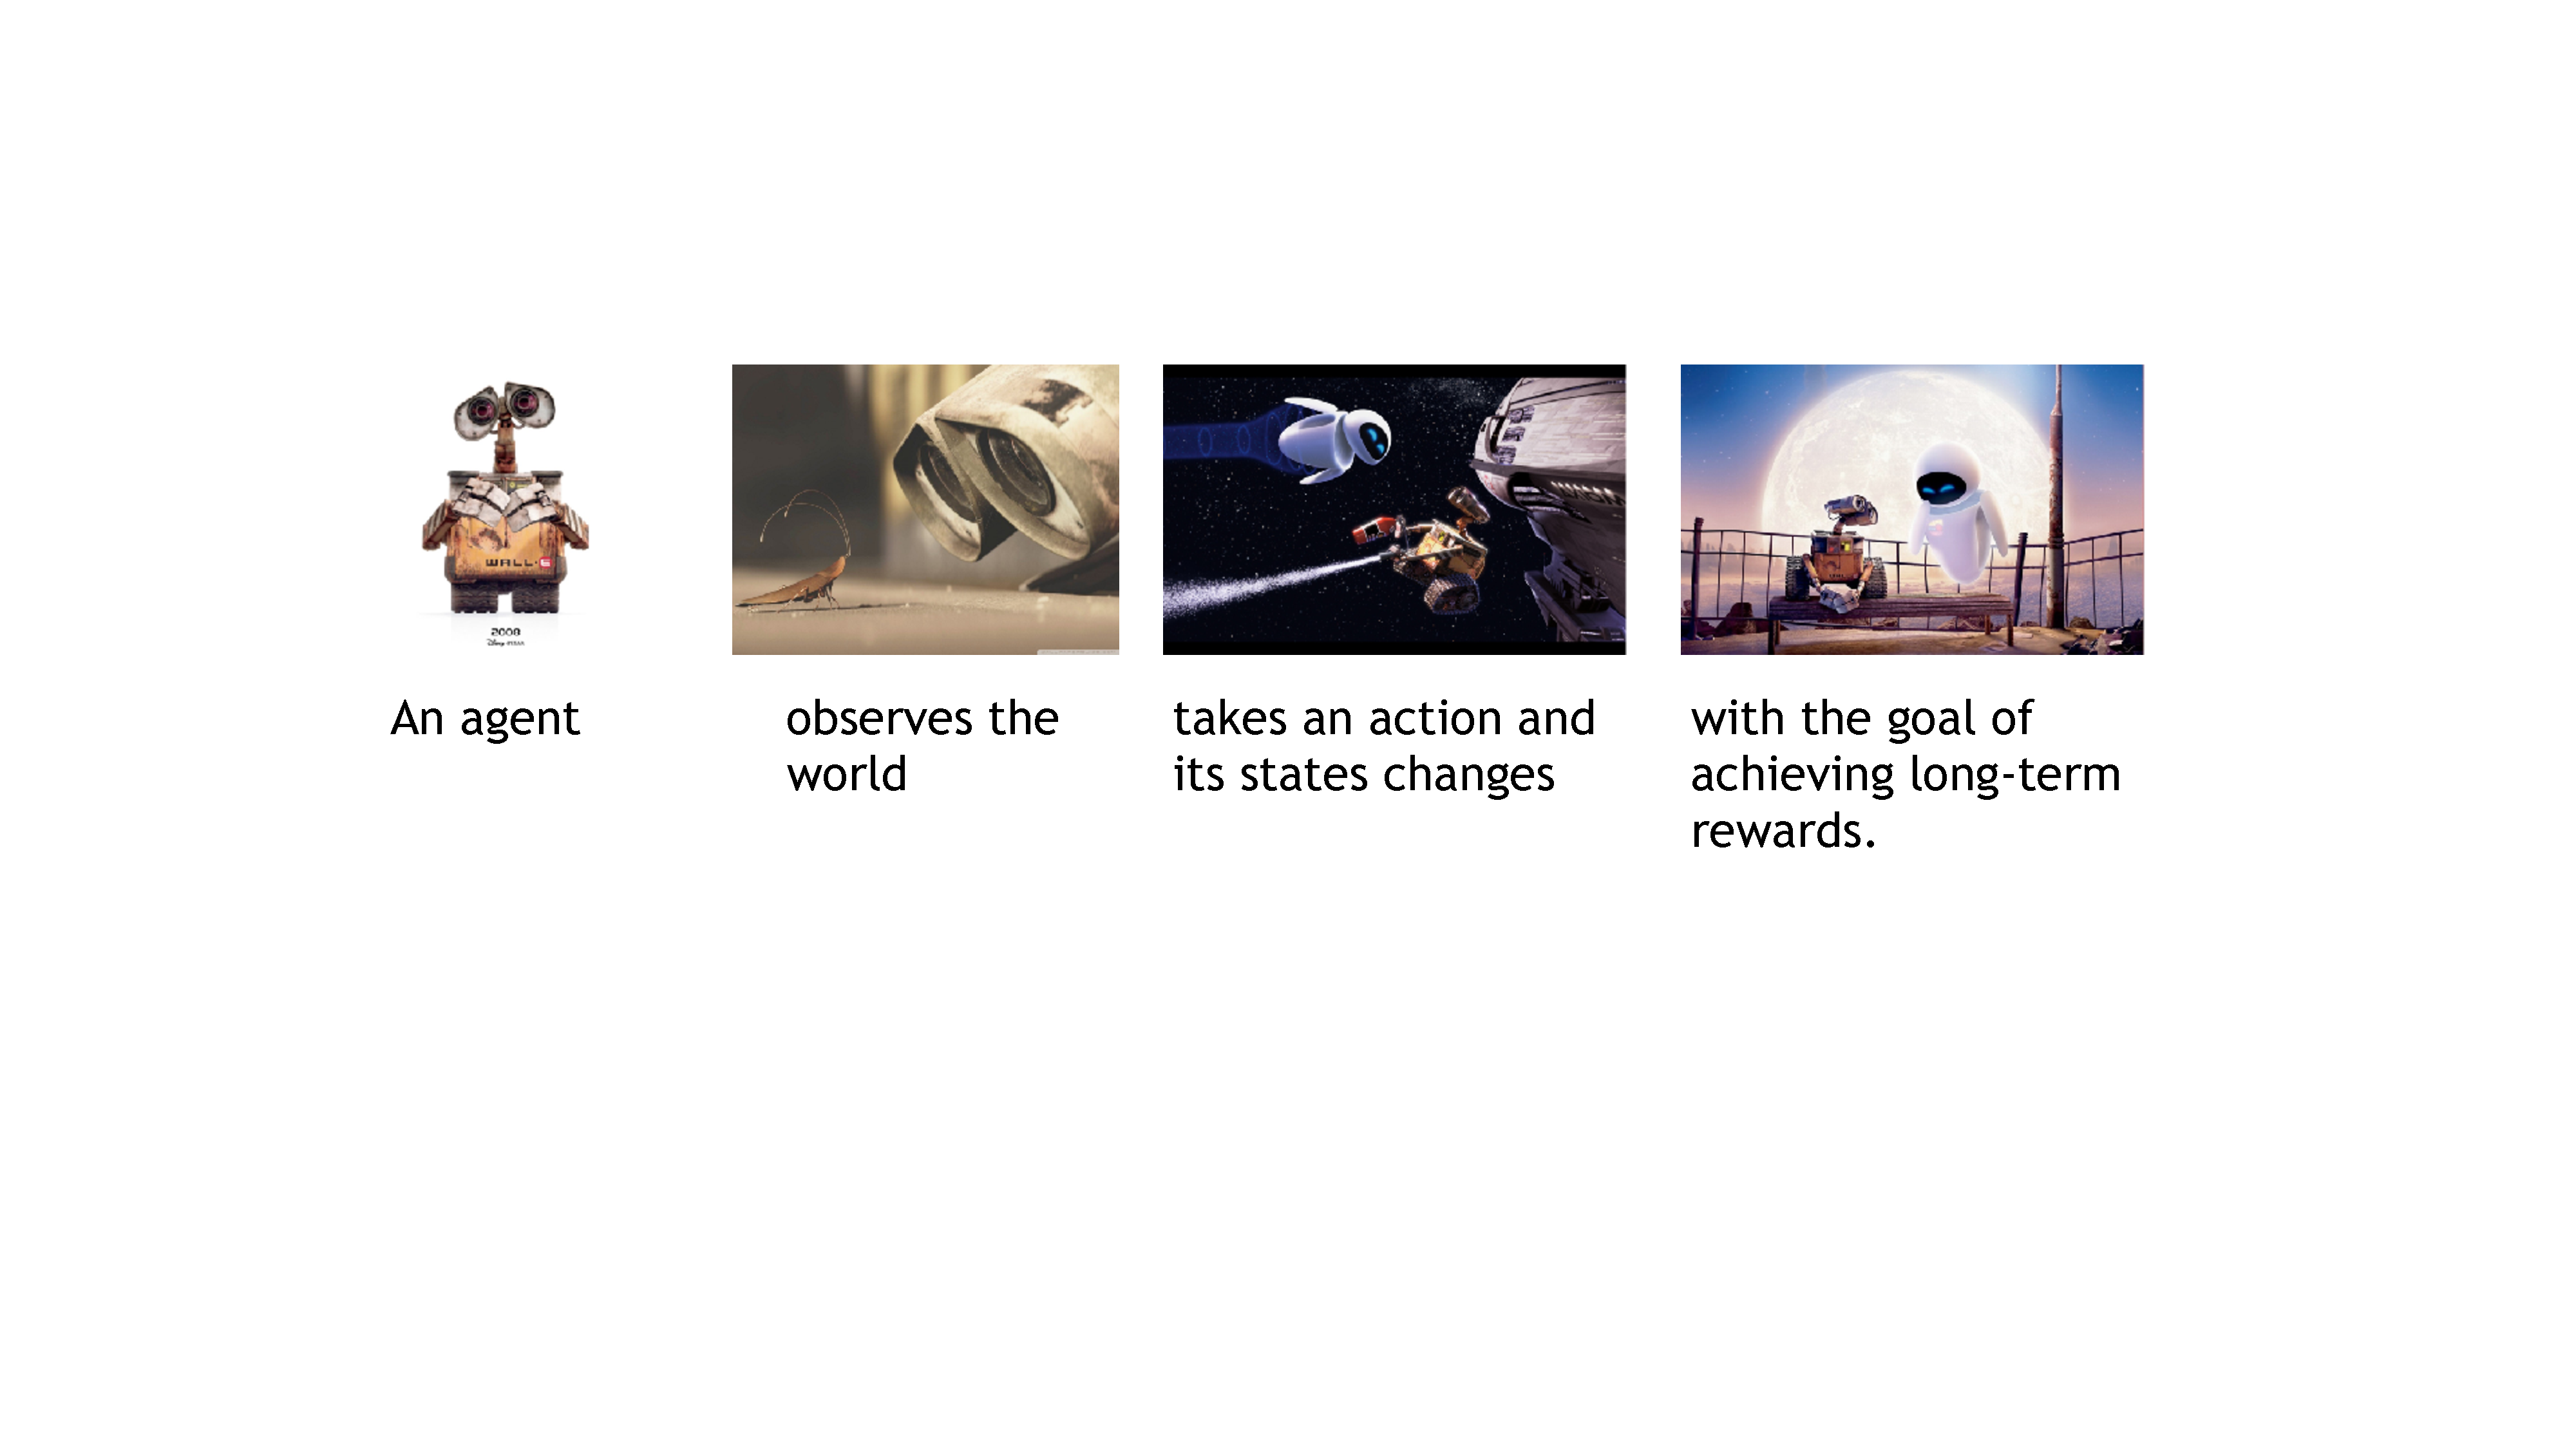
\includegraphics[width=0.75\linewidth]{Figures/RL_Problem}
\end{figure}

Reinforcement Learning Problem: An agent continually interacts with the environment. How should it choose its actions so that its long-term rewards are maximized?	
\end{frame}



%%%%%%%%%%%%%%%%%%%%%%%%%%%%%%%%%%%%%%%%%%%% 

\begin{frame}\frametitle{Playing Games: Atari}\small
\begin{figure}
\href{run:videos/intro/deep_mind.mp4}{
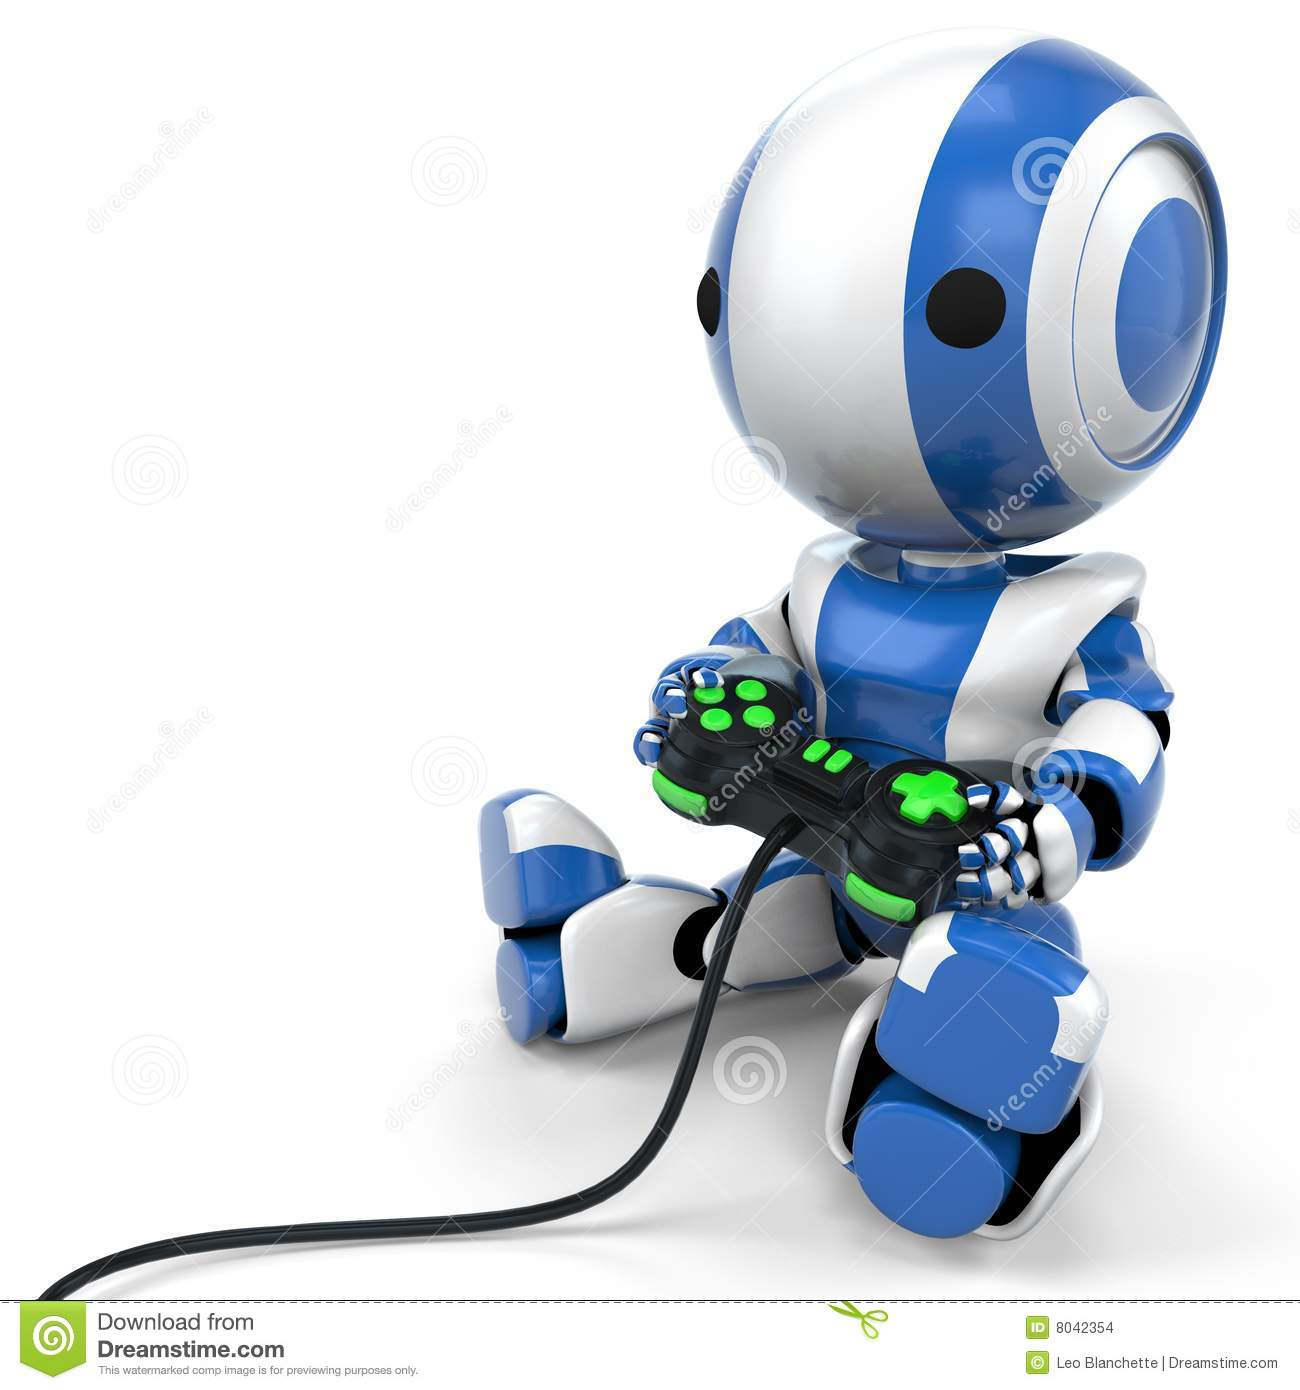
\includegraphics[width =0.6\linewidth,trim=0 69 0 0,clip]{Figures/robot_game.jpg}\\
{\color{magenta}{\url{https://www.youtube.com/watch?v=V1eYniJ0Rnk}}}
}
\end{figure}
\end{frame}

\begin{frame}\frametitle{Playing Games: Super Mario}\small
\begin{figure}
\href{run:videos/intro/super_mario.mp4}{
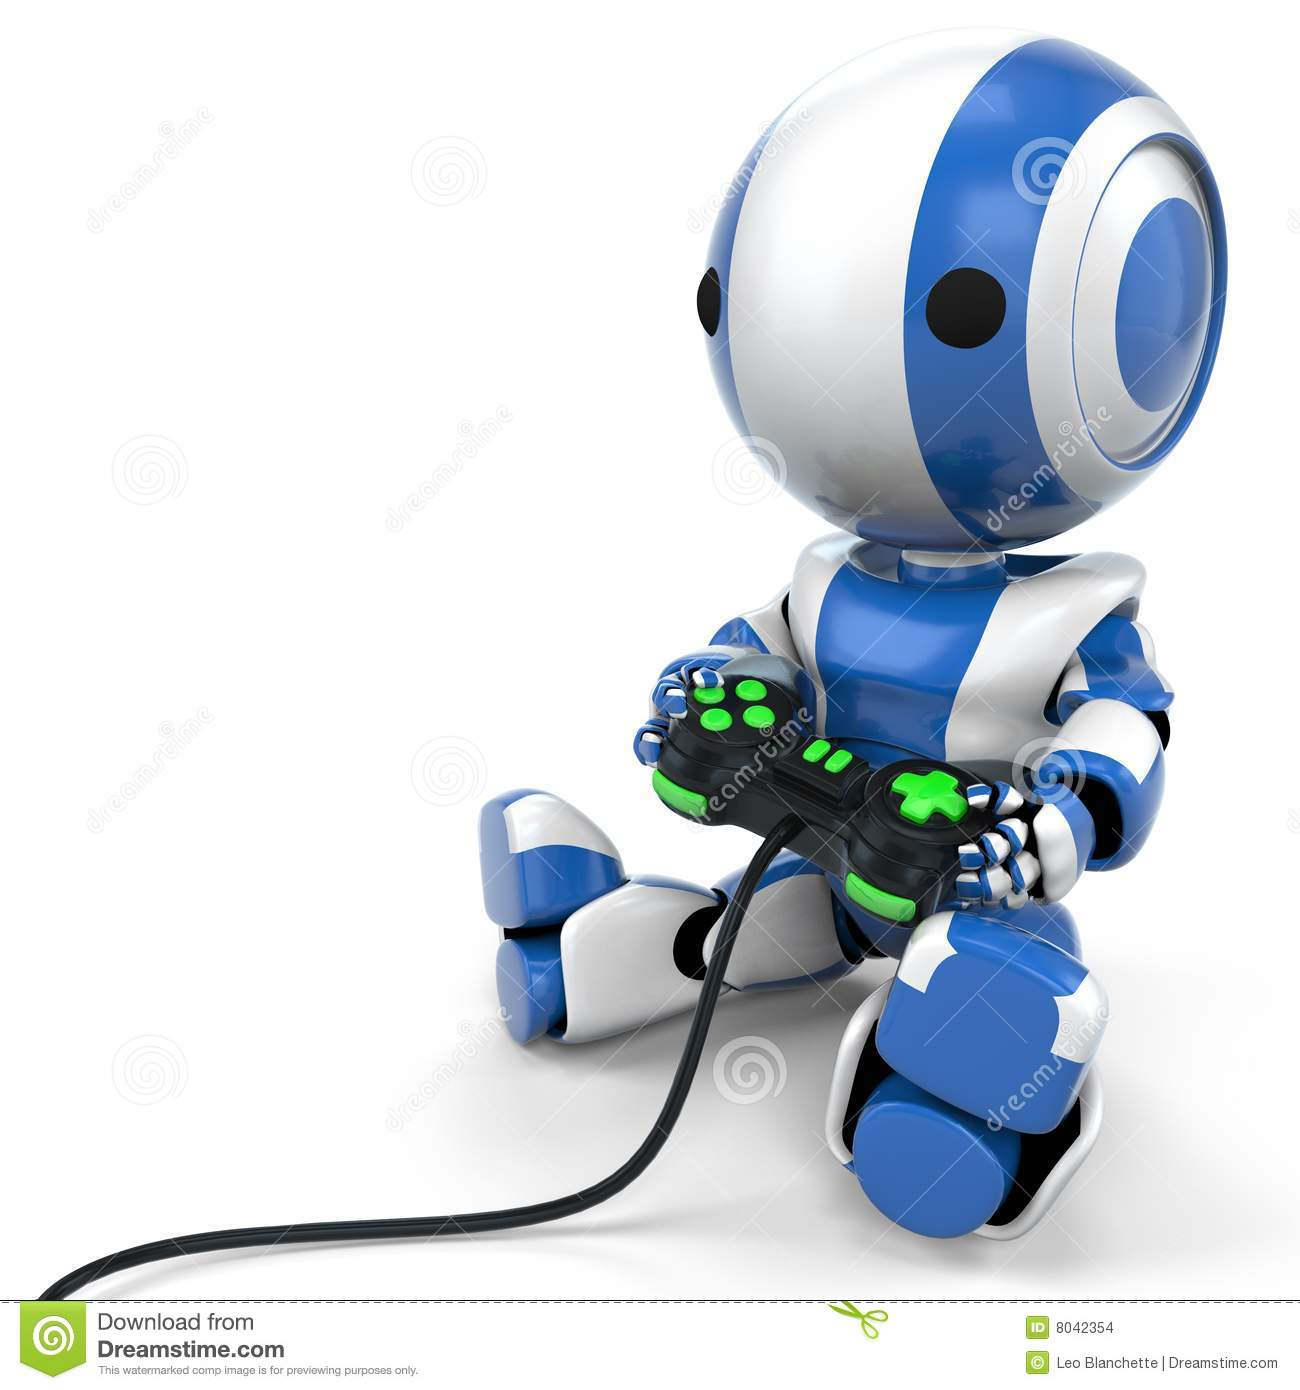
\includegraphics[width =0.6\linewidth,trim=0 69 0 0,clip]{Figures/robot_game.jpg}\\
{\color{magenta}{\url{https://www.youtube.com/watch?v=wfL4L_l4U9A}}}
}
\end{figure}
\end{frame}

\begin{frame}\frametitle{Making Pancakes!}\small
\begin{figure}
\href{run:videos/lecture19/pancakes.mp4}{
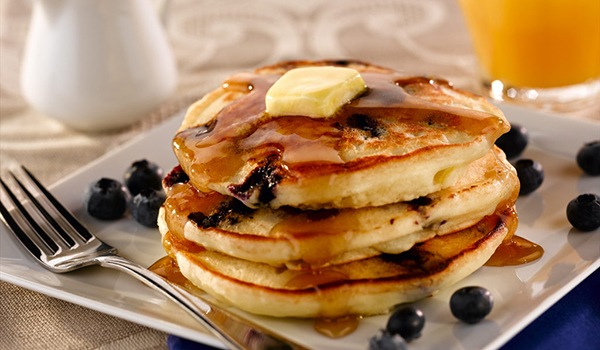
\includegraphics[width=0.9\linewidth]{Figures/pancakes1}\\
{\color{magenta}{\url{https://www.youtube.com/watch?v=W_gxLKSsSIE}}}
}
\end{figure}
\end{frame}


\begin{frame}\frametitle{Reinforcement Learning Resources}\small
\begin{itemize}

\item {\it Reinforcement Learning: An Introduction second edition}, Sutton \& Barto Book (2018)
\item  \href{https://www.youtube.com/watch?v=2pWv7GOvuf0}{Video lectures by David Silver}
\end{itemize}
\end{frame}

% \begin{frame}\frametitle{What is Reinforcement Learning?}\small
% \begin{figure}
% 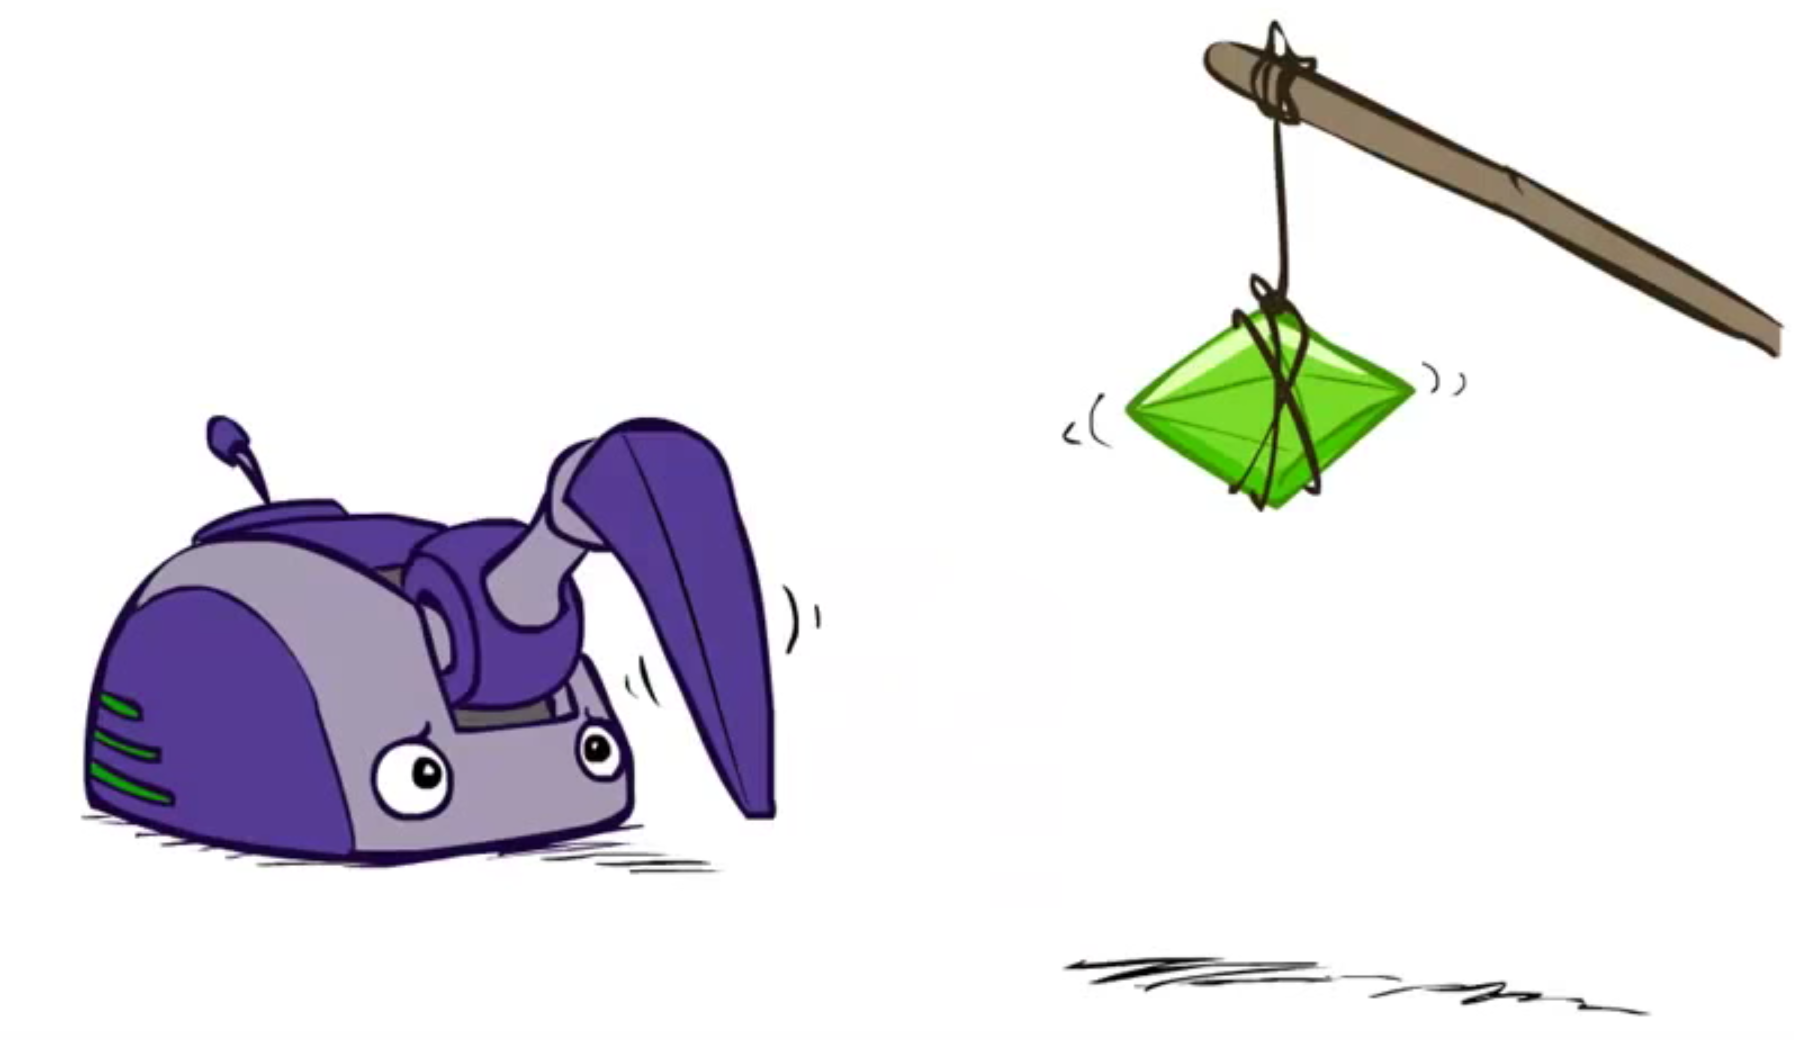
\includegraphics[width=0.9\linewidth]{../old_course_material/slides/figs/lecture19/rll2}
% \end{figure}
% \vspace{5mm}
% \scriptsize [pic from: Peter Abbeel]
% \end{frame}
% 

\begin{frame}\frametitle{Reinforcement Learning}\small
\begin{itemize}
\item Learning algorithms differ in the information available to learner
\begin{itemize}
\setlength\itemsep{1em}
\onslide<2->\item \high{Supervised}: correct outputs, e.g., class label
\onslide<3->\item \high{Unsupervised}: no feedback, must construct measure of good output
\onslide<4->\item \high{Reinforcement learning}: Reward (or cost)
\end{itemize}
\onslide<5->\item More realistic learning scenario: 
\begin{itemize}
\setlength\itemsep{1em}
\item Continuous stream of input information, and actions\\[0.7mm] 
\onslide<6->\item Effects of action depend on state of the world\\[0.7mm] 
\onslide<7->\item Obtain reward that depends on world state and actions\\[0.7mm] 
\begin{itemize}
\onslide<8->\item You know the reward for your action, not other actions.
\onslide<9->\item Could be a delay between action and reward.
\end{itemize}
\end{itemize}
\end{itemize}
\end{frame}

\begin{frame}\frametitle{Reinforcement Learning}\small
%\vspace{8mm}

\begin{figure}
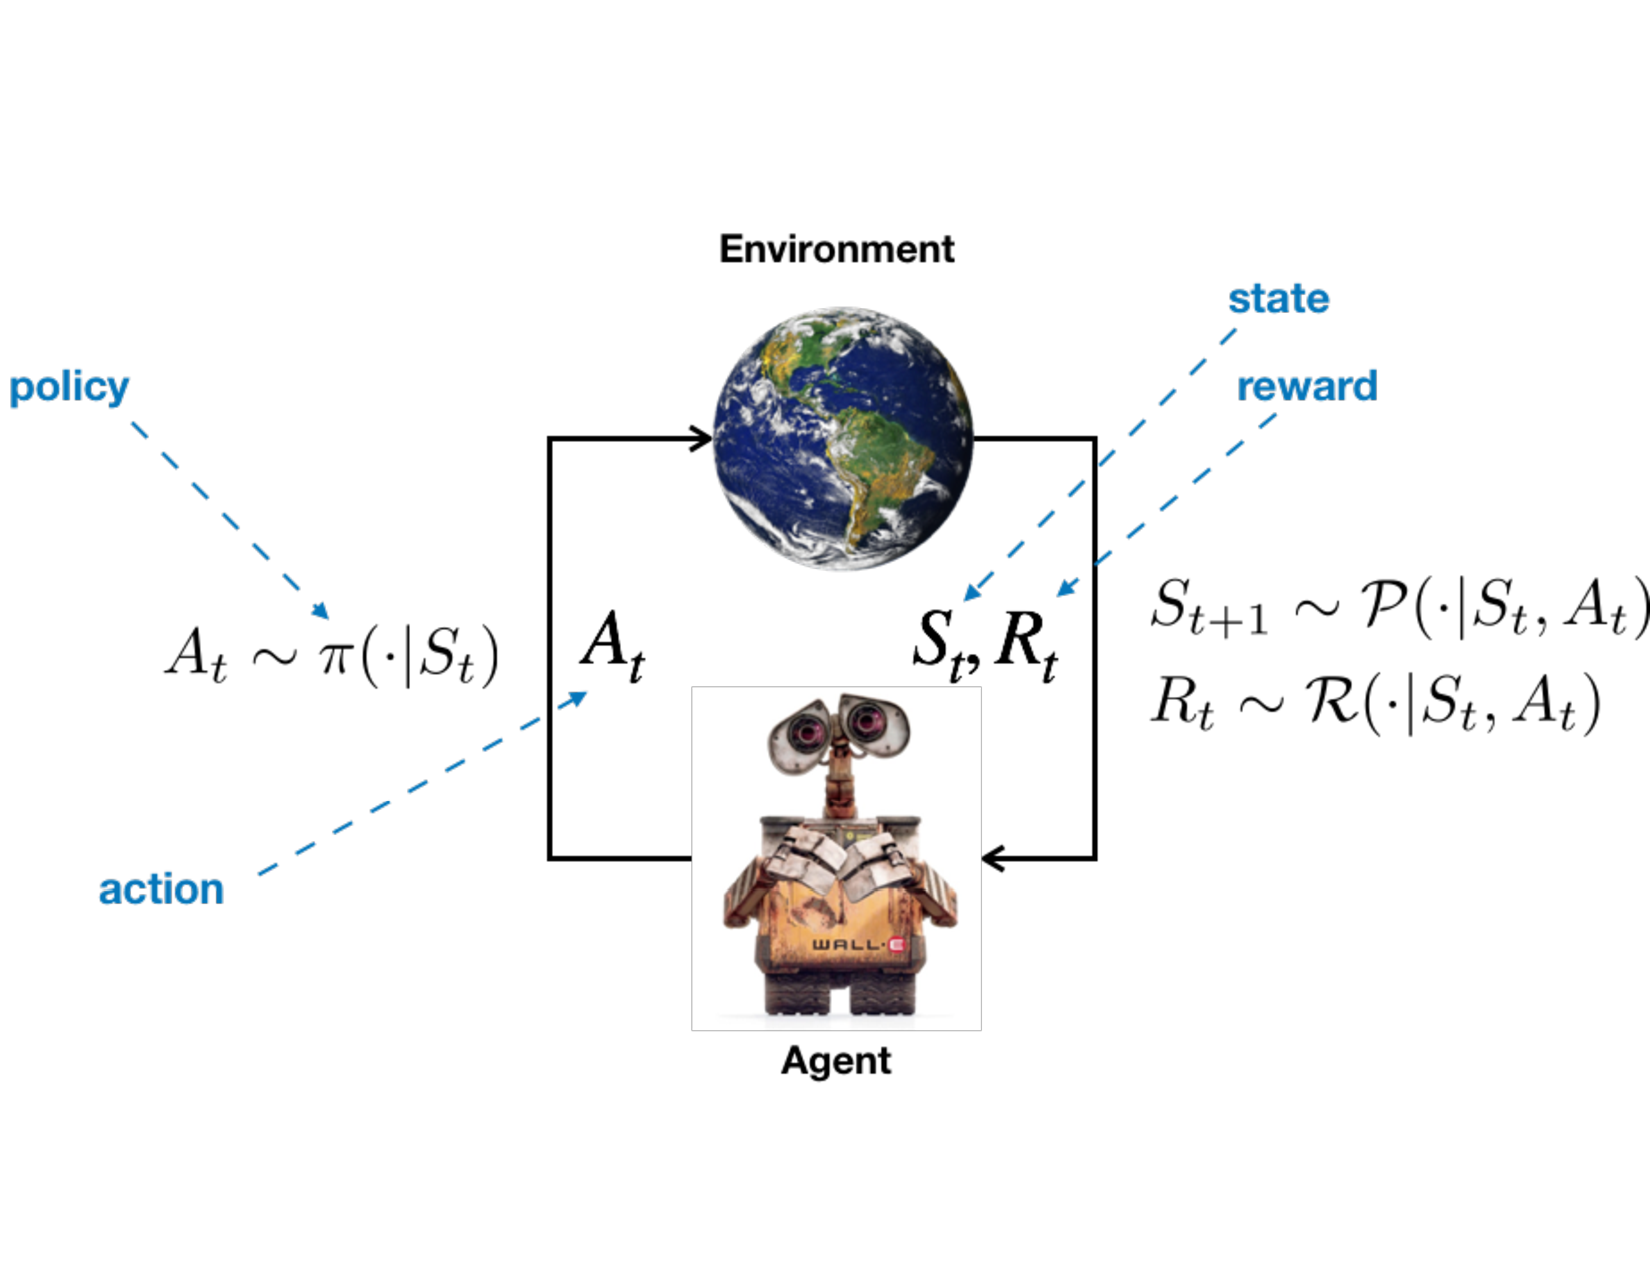
\includegraphics[width=0.85\linewidth]{Figures/RL_agent}
\end{figure}

%\begin{figure}
%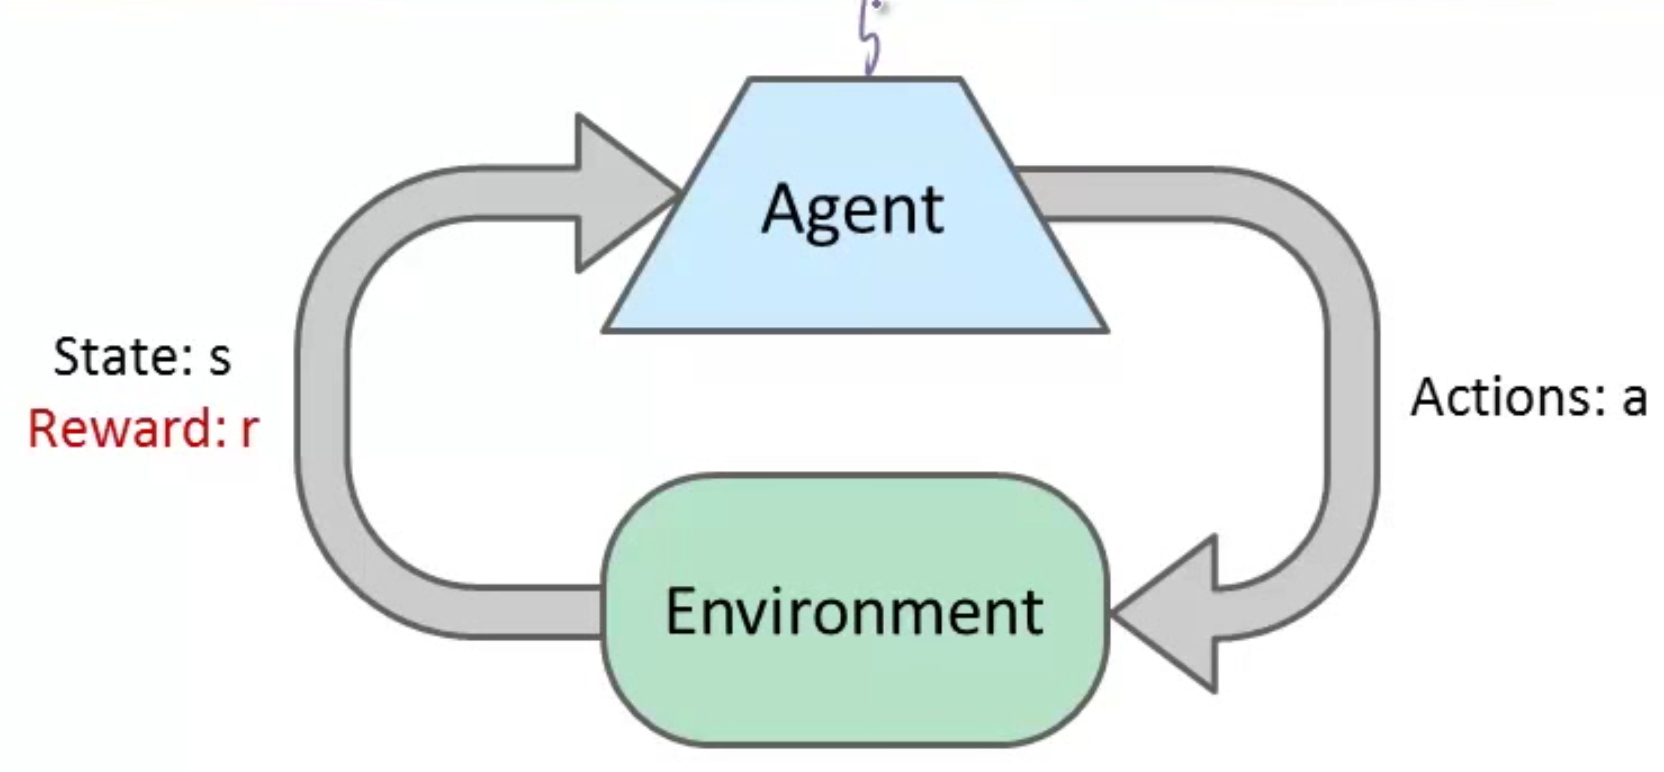
\includegraphics[width=0.85\linewidth]{Figures/rll3}
%\end{figure}
%\vspace{7mm}
%
%\scriptsize [pic from: Peter Abbeel]
\end{frame}

\begin{frame}\frametitle{Example: Tic Tac Toe, Notation}\small
\vspace{4mm}
\begin{figure}
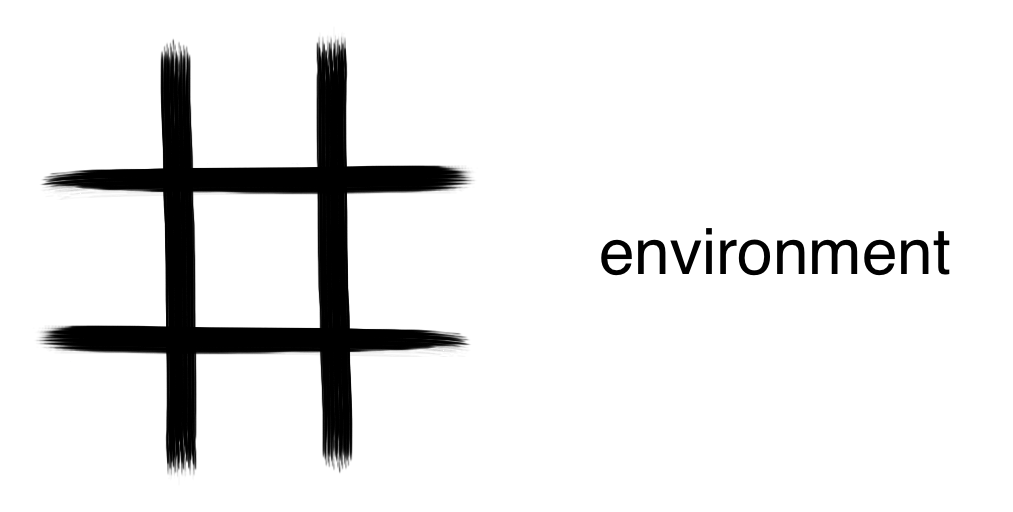
\includegraphics[width=0.75\linewidth]{Figures/tic1d}
\end{figure}
\vspace{5mm}
\end{frame}

\begin{frame}\frametitle{Example: Tic Tac Toe, Notation}\small
\vspace{4mm}

\begin{figure}
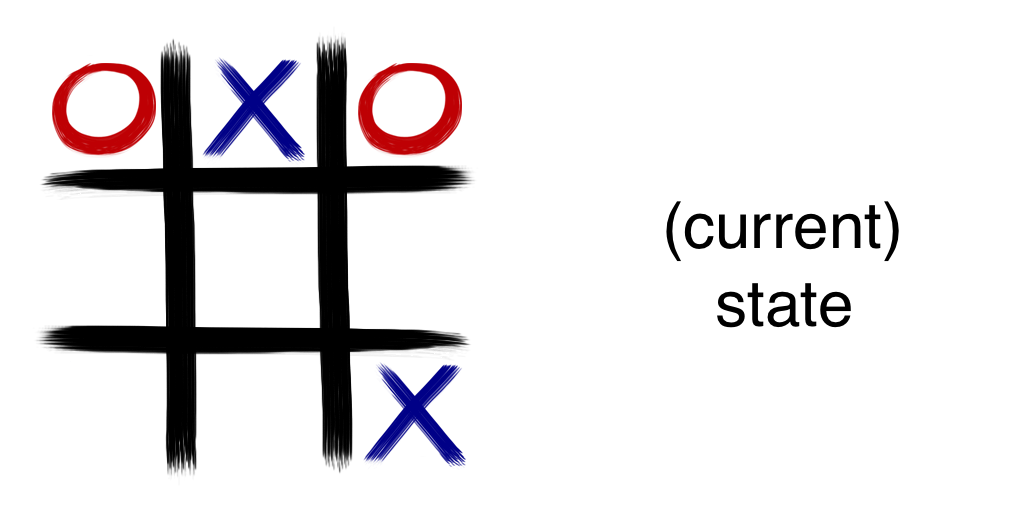
\includegraphics[width=0.75\linewidth]{Figures/tic1c}
\end{figure}
\vspace{5mm}
\end{frame}

\begin{frame}\frametitle{Example: Tic Tac Toe, Notation}\small
\vspace{4mm}

\begin{figure}
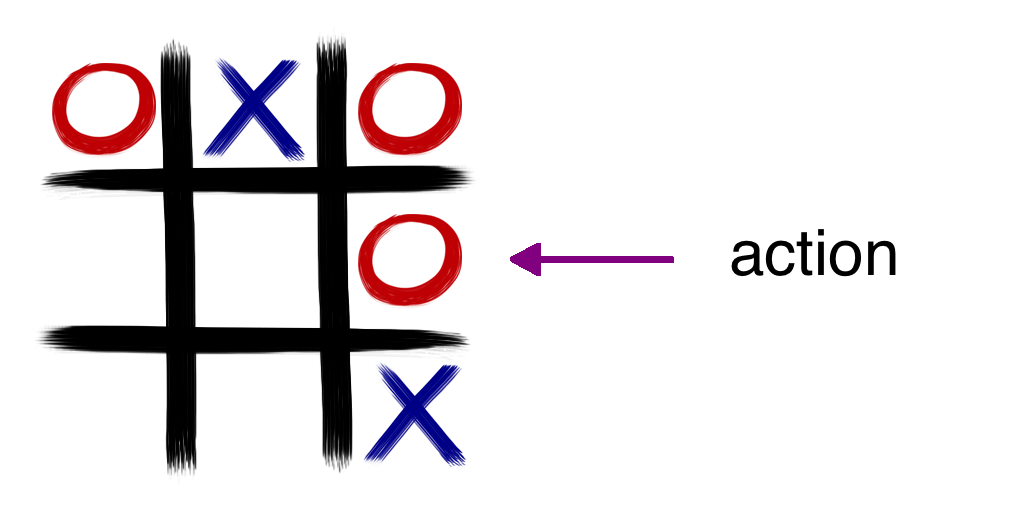
\includegraphics[width=0.75\linewidth]{Figures/tic1b}
\end{figure}
\vspace{5mm}
\end{frame}

\begin{frame}\frametitle{Example: Tic Tac Toe, Notation}\small
\vspace{4mm}

\begin{figure}
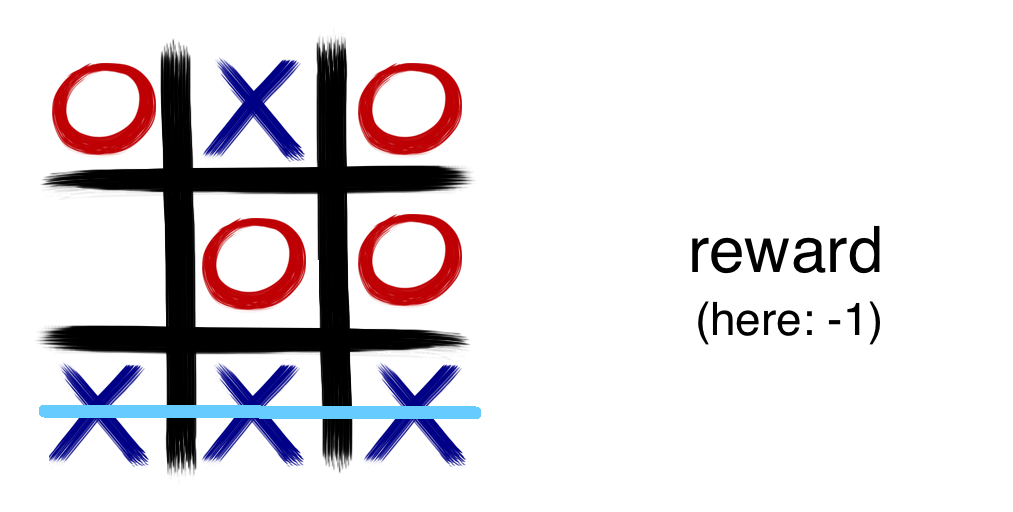
\includegraphics[width=0.75\linewidth]{Figures/tic1e}
\end{figure}
\vspace{5mm}
\end{frame}


%%%%%%%%%%%%%%%%%%%%%%%%%%%%%%%%%%%%%%%%%%%% 
\begin{frame}\frametitle{Formalizing Reinforcement Learning Problems}\small
\begin{itemize}
\item Markov Decision Process (MDP) is the mathematical framework to describe RL problems
\item A discounted MDP is defined by a tuple $(\States, \Actions, \PKernel, \RKernel, \gamma)$.
\begin{itemize}
	\item $\States$: State space. Discrete or continuous
	\item $\Actions$: Action space. Here we consider finite action space, i.e., $\Actions = \{a_1, \dotsc, a_{|\Actions|} \}$.
	\item $\PKernel$: Transition probability
	\item $\RKernel$: Immediate reward distribution
	\item $\gamma$: Discount factor ($0 \leq \gamma < 1$)
\end{itemize}
\end{itemize}

\end{frame}


%%%%%%%%%%%%%%%%%%%%%%%%%%%%%%%%%%%%%%%%%%%% 
\begin{frame}\frametitle{Formalizing Reinforcement Learning Problems}\small
\begin{itemize}
\item The agent has a \high{state} $s \in \mathcal{S}$ in the environment, e.g., the location of X and O in tic-tac-toc, or the location of a robot in a room.
\item At every time step $t = 0, 1, \dotsc$, the agent is at state $s_t$.
	\begin{itemize}
	\item Takes an \high{action} $a_t$
	\item Moves into a new state $s_{t+1}$, according to the dynamics of the environment and the selected action, i.e., $s_{t+1} \sim \PKernel(\cdot|s_t, a_t)$
	\item Receives some \high{reward} $r_{t+1} \sim \RKernel(\cdot|s_t, a_t, s_{t+1})$
	\end{itemize}
\end{itemize}
\begin{figure}
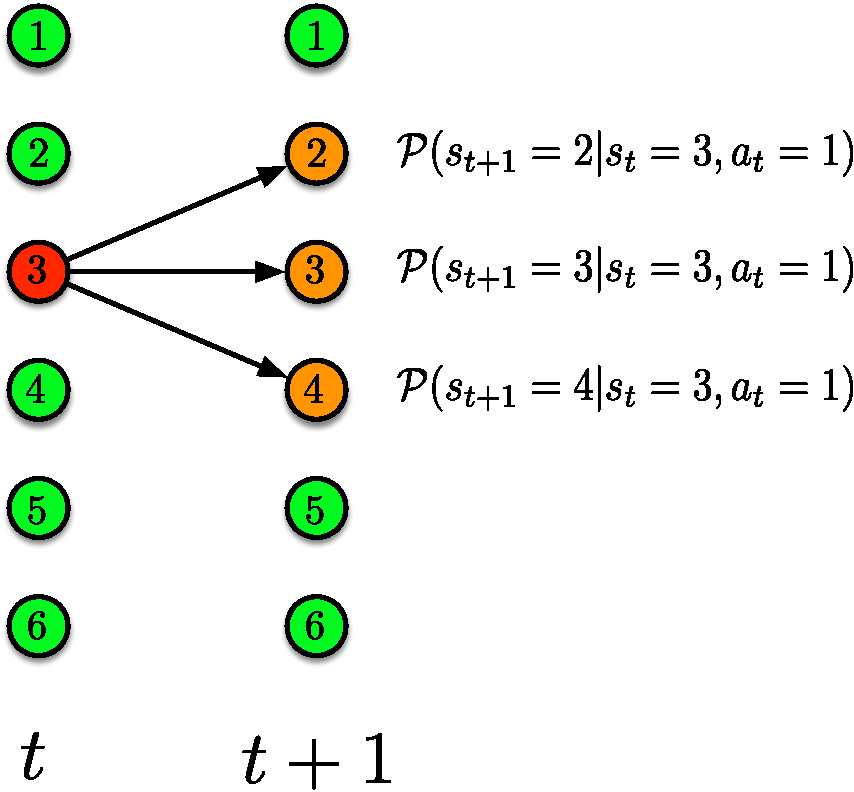
\includegraphics[width=0.3\linewidth]{Figures/MDP_transition}
\end{figure}
\end{frame}




%%%%%%%%%%%%%%%%%%%%%%%%%%%%%%%%%%%%%%%%%%%% 
\begin{frame}\frametitle{Formulating Reinforcement Learning}\small

%\begin{figure}
%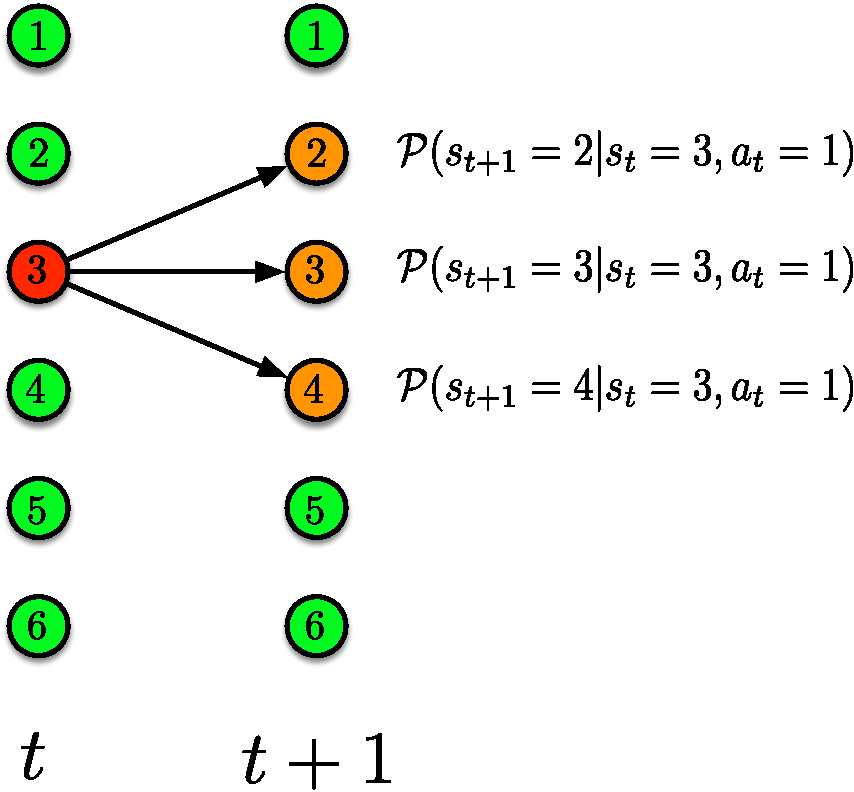
\includegraphics[width=0.1\linewidth]{Figures/MDP_transition}
%\end{figure}

\begin{itemize}
\item The action selection mechanism is described by a \high{policy} $\pi$
\begin{itemize}
\item Policy $\pi$ is a mapping from states to actions, i.e., $a_t = \pi(s_t)$
\end{itemize}
\item The goal is to find a policy $\pi$ such that \high{long-term rewards} of the agent is maximized. 
\item Different notations of long-term reward:
	\begin{itemize}
	\item
	Average reward:
	\[
	r_{t}+r_{t+1}+r_{t+2}+\dots
	\]
	\item Sometimes a future reward is discounted by $\gamma^{k-1}$, where $k$ is the number of time-steps in the future when it is received:
		\[
	r_{t}+\gamma r_{t+1}+\gamma^2 r_{t+2}+\dots
	\]
		\begin{itemize}
			\item If $\gamma$ close to $1$, rewards further in the future count more, and we say that the agent is ``farsighted''
			\item $\gamma$ is less than $1$ because there is usually a time limit to the sequence of actions needed to solve a task (we prefer rewards sooner rather than 
		\end{itemize}
	\end{itemize}
\end{itemize}
\end{frame}


%%%%%%%%%%%%%%%%%%%%%%%%%%%%%%%%%%%%%%%%%%% 
\begin{frame}\frametitle{Transition Probability (or Dynamics)}\small
\begin{itemize}
\item The transition probability describes the changes in the state of the agent when it chooses actions
\[
	\PKernel(s_{t+1}=s', r_{t+1}=r' | s_t = s, a_t = a)
\]
%
\item This model has \high{Markov property}: the future depends on the past only through the current state
%
\end{itemize}
\begin{figure}
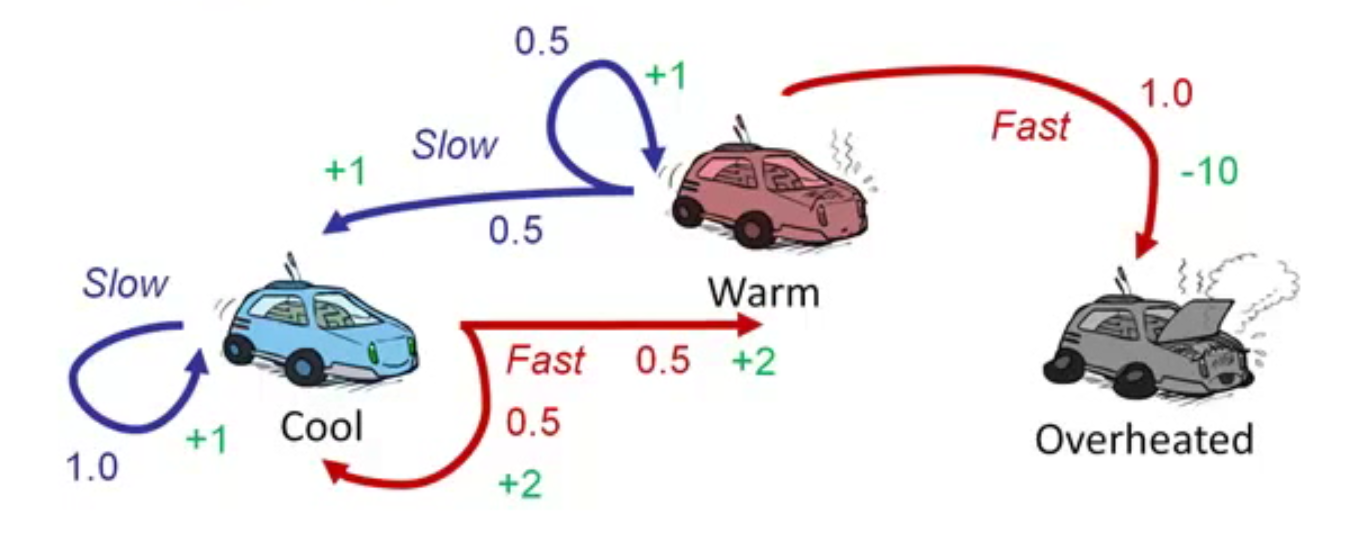
\includegraphics[width=0.7\linewidth]{Figures/rll6} 
\end{figure}
\end{frame}


%%%%%%%%%%%%%%%%%%%%%%%%%%%%%%%%%%%%%%%%%%% 
\begin{frame}\frametitle{Policy}\small
\begin{itemize}
\item A \high{policy} is the action selection mechanism of the agent, and describes its behaviour.
\item Policy can be deterministic or stochastic:
	\begin{itemize}
		\item Deterministic policy: $a = \pi(s)$
		\item Stochastic policy: $A \sim \pi(\cdot|s)$
	\end{itemize}
\end{itemize}
\end{frame}


%%%%%%%%%%%%%%%%%%%%%%%%%%%%%%%%%%%%%%%%%%% 
\begin{frame}\frametitle{Value Function}\small
\begin{itemize}
\item \high{Value function} is the expected future reward, and is used to evaluate the desirability of states.
\item State-value function $\Vpi$ (or simply value function) for policy $\pi$ is a function defined as
\begin{align*}
	\Vpi(s) \eqdef \EEX{\pi}{\sum_{t \geq 0} \gamma^t R_t \mid S_0 = s}.
\end{align*}
It describes the expected discounted reward if the agent starts from state $s$ and follows policy $\pi$.

\item The action-value function $\Qpi$ for policy $\pi$ is
\begin{align*}
	\Qpi(s,a) \eqdef \EEX{\pi}{\sum_{t \geq 0} \gamma^t R_t \mid S_0 = s, A_0 = a}.
\end{align*}
It describes the expected discounted reward if the agent starts from state $s$, takes action $a$, and afterwards follows policy $\pi$.
\end{itemize}
\end{frame}

%%%%%%%%%%%%%%%%%%%%%%%%%%%%%%%%%%%%%%%%%%% 
\begin{frame}\frametitle{Value Function}\small

\begin{itemize}
	\item Our aim will be to find a policy $\pi$ that maximizes the value function (the total reward we receive over time): find the policy with the highest expected reward
	\item Optimal value function:
	\[
	  \Qopt(s,a) = \sup_\pi \Qpi(s,a)
	\]

	\item Given $\Qopt$, the optimal policy can be obtained as
	\[
	  \piopt(s) \leftarrow \argmax_a \Qopt(s,a)
	\]

	\item The goal of an RL agent is to find a policy $\pi$ that is close to optimal, i.e., $\Qpi \approx \Qopt$.
\end{itemize}
\end{frame}



%%%%%%%%%%%%%%%%%%%%%%%%%%%%%%%%%%%%%%%%%%% 
\begin{frame}\frametitle{Bellman Equation}\small
The value function satisfies the following recursive relationship:
\begin{align*}
  \Qpi(s,a) & = \EE{\sum_{t=0}^\infty \gamma^t R_t | S_0 = s, A_0 = a }
  \\
  &
  = \EE{R(S_0, A_0) + \gamma \sum_{t = 0}^\infty \gamma^t R_{t+1} | s_0 = s, a_0 = a }
  \\
  &  
  = \EE{R(S_0, A_0) + \gamma \Qpi(S_1, \pi(S_1)) | S_0 = s, A_0 = a }
  \\
  &
  =
  \underbrace{
  r(s,a) + \gamma \int_\States \PKernel(\ds' | s, a) \Qpi (s', \pi(s')) }_{\eqdef (\Tpi \Qpi)(s,a) }
\end{align*}
This is called the Bellman equation and $\Tpi: B(\SA) \ra B(\SA)$ is the Bellman operator.
Similarly, we define the Bellman \emph{optimality} operator:
\begin{align*}
  (\Topt Q)(s,a) \eqdef r(s,a) + \gamma \int_\States \PKernel(\ds' | s,a) \max_{a' \in \Actions} Q(s',a')
\end{align*}
\end{frame}


%%%%%%%%%%%%%%%%%%%%%%%%%%%%%%%%%%%%%%%%%%% 
\begin{frame}\frametitle{Bellman Equation}\small
\begin{itemize}
	\item Key observation:
	\begin{align*}
	  & \Qpi = \Tpi \Qpi \\
	  & \Qopt = \Topt \Qopt
	\end{align*}

	\item Value-based approaches try to find a $\Qhat$ such that
	\[
	  \Qhat \approx \Topt \Qhat
	\]

	\item The greedy policy of $\Qhat$ is close to the optimal policy:
	\[
		  % Q^{\pi(x;\Qhat)} \approx Q^{\piopt} = \Qopt
		  Q^{\pi(x;\Qhat)} \approx \Qopt
	\]
	where the greedy policy is defined as
	\[
	  \pi(s; \Qhat) \leftarrow \argmax_{a \in \Actions} \Qhat(s,a)
	\]
\end{itemize}
\end{frame}


%%%%%%%%%%%%%%%%%%%%%%%%%%%%%%%%%%%%%%%%%%% 
\begin{frame}\frametitle{Finding the Optimal Value Function: Value Iteration}\small
\begin{itemize}
	\item Assume that we know the model $\PKernel$ and $\RKernel$. How can we find the optimal value function?
	\item This is the problem of \high{Planning}.
	\item We can benefit from the Bellman optimality equation and use a method called \high{Value Iteration}
		\[
			Q_{k+1} \leftarrow \Topt Q_k
		\]
	\begin{figure}
		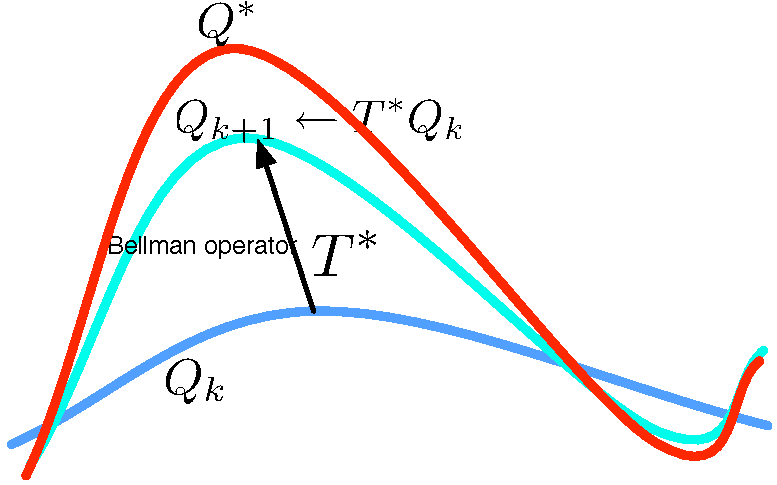
\includegraphics[width=0.4\linewidth]{Figures/VI} 
	\end{figure}
\end{itemize}
\vspace{-0.5cm}
\begin{align*}
	&
	Q_{k+1}(s,a) \leftarrow r(s,a) + \gamma \int_{\States} \PKernel(\ds' | s,a) \max_{a' \in \AA} Q_k(s',a')
	\\
	& Q_{k+1}(s,a) \leftarrow r(s,a) + \gamma \sum_{s' \in \States} \PKernel(s' | s,a) \max_{a' \in \AA} Q_k(s',a')
\end{align*}
\end{frame}


%%%%%%%%%%%%%%%%%%%%%%%%%%%%%%%%%%%%%%%%%%% 
\begin{frame}\frametitle{Value Iteration}\small
\begin{itemize}
	\item The Value Iteration converges to the optimal value function.
	\item This is because of the contraction property of the Bellman (optimality) operator, i.e., $\norm{\Topt Q_1 - \Topt Q_2}_\infty \leq \gamma \norm{Q_1 - Q_2}_\infty$.
\end{itemize}
	\begin{figure}
		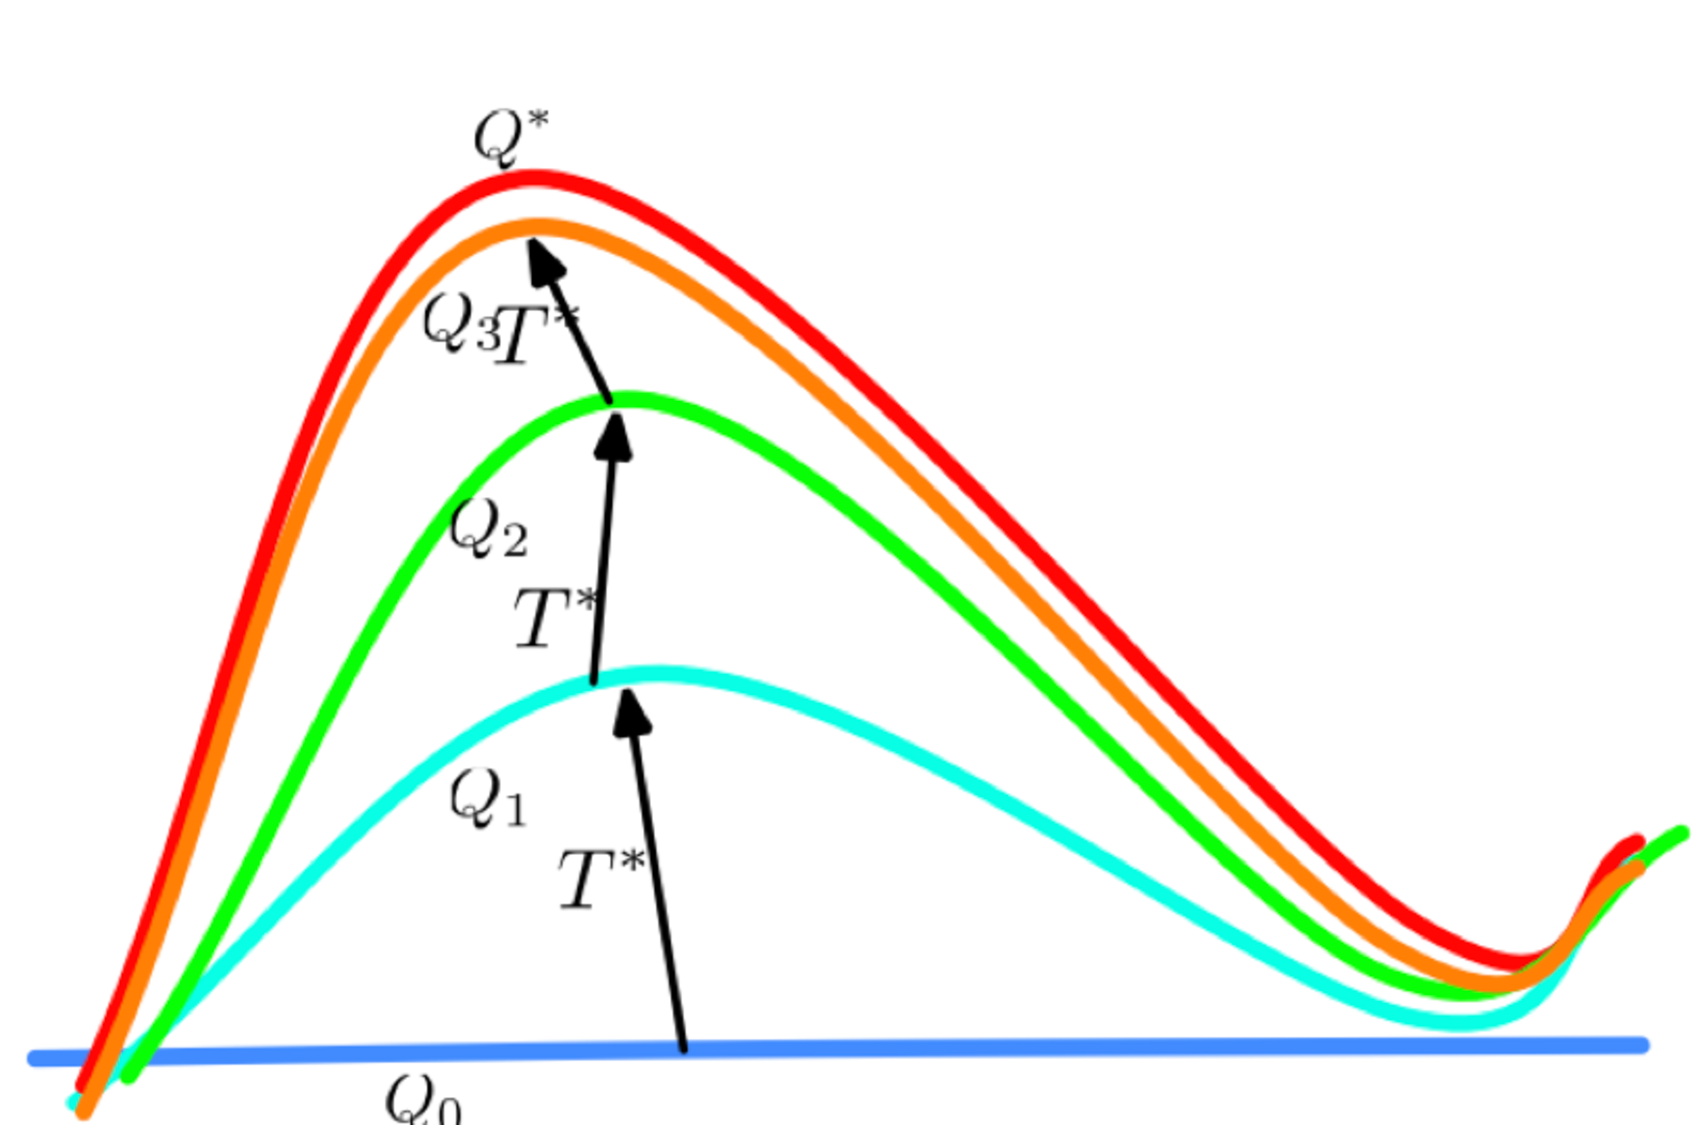
\includegraphics[width=0.4\linewidth]{Figures/VI_Convergence} 
		\vspace{-0.2in}
	\end{figure}
\[
	Q_{k+1} \leftarrow \Topt Q_k
\]
\begin{align*}
	&
	Q_{k+1}(s,a) \leftarrow r(s,a) + \gamma \int_{\States} \PKernel(\ds' | s,a) \max_{a' \in \AA} Q_k(s',a')
	\\
	& Q_{k+1}(s,a) \leftarrow r(s,a) + \gamma \sum_{s' \in \States} \PKernel(s' | s,a) \max_{a' \in \AA} Q_k(s',a')
\end{align*}
\end{frame}

\begin{frame}\frametitle{Maze Example}\small
\begin{figure}
\begin{minipage}{0.5\linewidth}
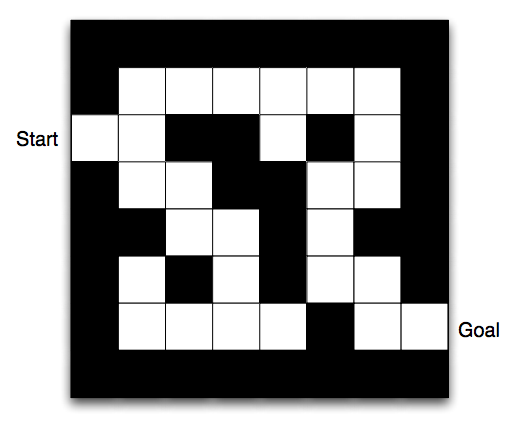
\includegraphics[width=\linewidth]{Figures/maze1}
\end{minipage}
\hspace{3mm}
\begin{minipage}{0.45\linewidth}
\begin{itemize}
\item Rewards: \onslide<2-> $-1$ per time-step
\item Actions: \onslide<3-> N, E, S, W
\item States: \onslide<4-> Agent's location
\end{itemize}
\end{minipage}
\end{figure}

\vspace{12mm}
\scriptsize [Slide credit: D. Silver]
\end{frame}

\begin{frame}\frametitle{Maze Example}\small
\begin{figure}
\begin{minipage}{0.5\linewidth}
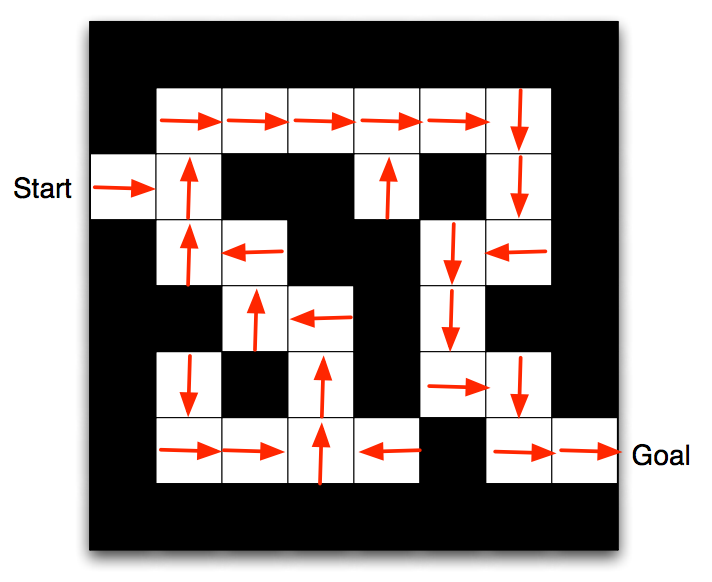
\includegraphics[width=\linewidth]{Figures/maze2}
\end{minipage}
\hspace{3mm}
\begin{minipage}{0.45\linewidth}
\begin{itemize}
\item Arrows represent policy $\pi(s)$ for each state $s$
\end{itemize}
\end{minipage}
\end{figure}

\vspace{14mm}
\scriptsize [Slide credit: D. Silver]
\end{frame}

\begin{frame}\frametitle{Maze Example}\small
\begin{figure}
\begin{minipage}{0.5\linewidth}
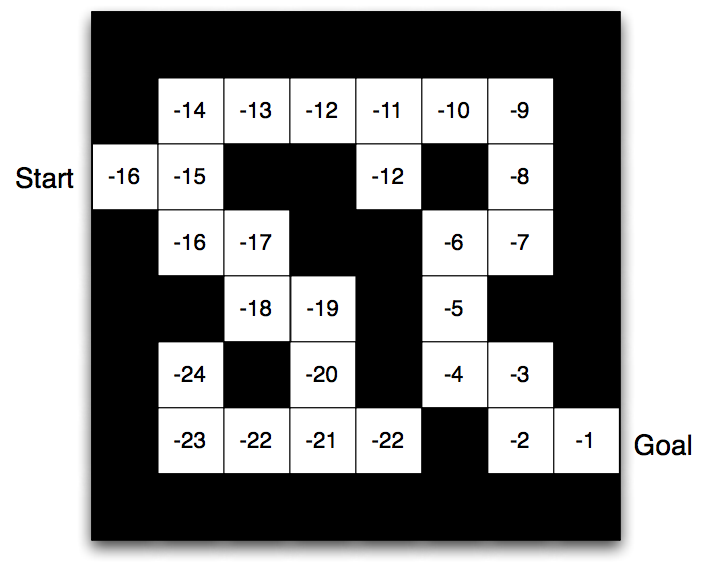
\includegraphics[width=\linewidth]{Figures/maze3}
\end{minipage}
\hspace{3mm}
\begin{minipage}{0.45\linewidth}
\begin{itemize}
\item Numbers represent value $V^{\pi}(s)$ of each state $s$
\end{itemize}
\end{minipage}
\end{figure}
\vspace{14mm}
\scriptsize [Slide credit: D. Silver]
\end{frame}

\begin{frame}\frametitle{Example: Tic-Tac-Toe}\small
\begin{itemize}
\item Consider the game tic-tac-toe:
\begin{itemize}
 \setlength\itemsep{1em}
\onslide<2->\item \high{reward}: \onslide<3-> win/lose/tie the game $(+1/-1/0)$ [only at final move in given game]
\onslide<4->\item \high{state}: \onslide<5->positions of X's and O's on the board
\onslide<6->\item \high{policy}: mapping from states to actions 
\begin{itemize}
\onslide<7->\item based on rules of game: choice of one open position
\end{itemize}
\onslide<8->\item \high{value function}: prediction of reward in future, based    on current state
\end{itemize}
\onslide<9->\item In tic-tac-toe, since state space is tractable, we can use a table to represent value function 
\end{itemize}
\end{frame}

\begin{frame}\frametitle{RL \& Tic-Tac-Toe}\small
%\vspace{-0.3cm}
\begin{itemize}
\item Each board position (taking into account symmetry) has some probability
\end{itemize}
\begin{minipage}{4cm}
\begin{center}
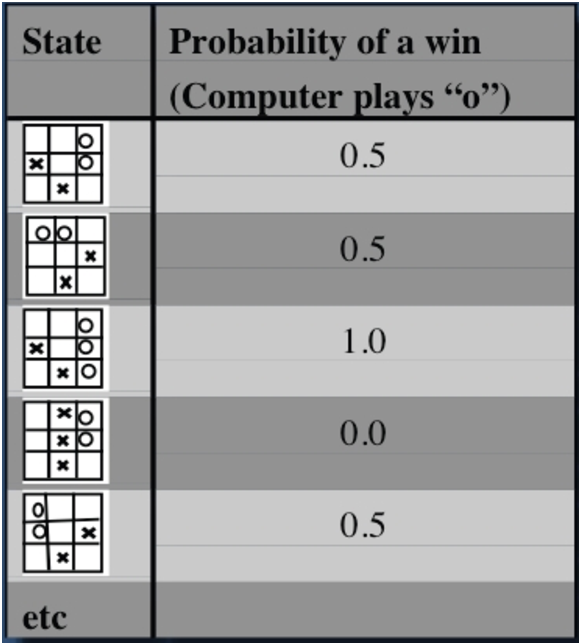
\includegraphics[width=1.0\linewidth]{Figures/tic_tac} 
\end{center}
\end{minipage}
\begin{minipage}{7cm}
\begin{itemize}
%\item Each board position (taking into account symmetry) has some probability
\onslide<2->\item Simple learning process: 
\begin{itemize}
\onslide<3->\item start with all values = 0.5
\onslide<4->\item \high{policy}: choose move with highest probability of winning given current legal moves from current state
\onslide<5->\item update entries in table based on outcome of each game
\onslide<6->\item After many games value function will represent true probability of winning from each state
\end{itemize}
%\item Can try alternative policy: sometimes select moves randomly (exploration)
\end{itemize}
\end{minipage}
\begin{itemize}
\onslide<7->\item Can try alternative policy: sometimes select moves randomly (exploration)
\end{itemize}
\end{frame}

\end{document}